
%%%%%%%%% PROPOSAL -- 15 pages (including Results from Prior NSF Support)

\noindent{\large\bf Social Robot Learning Companions for Personalized Children's Education}

\section{Introduction \& Problem Definition}
Social-robot learning companions have great potential to augment the efforts of parents and teachers to promote learning, academic knowledge, and the wellbeing of children. Interactions between a child and a robot resemble the speech acts between children and adults or peers, and offer a unique opportunity to personalize social interactions to promote early literacy skills.
 
However, the lack of reliable tools for analyzing children's speech is a major impediment to the further development and widespread deployment of truly impactful social robot tutors. Other barriers are rapidly falling: robust, affordable, and capable social robot platforms are beginning to enter the consumer market. Cloud-based infrastructure for data and computing are mature and accessible to all. Ordinary people interact daily with speech-based interfaces. Companies have recognized the importance of speech science, AI, and robotics as technologies of the future and are investing in their advancement accordingly. The time is ripe to develop the speech tools, algorithms, and models necessary to unlock the full potential of networked social robot systems to engage children and help promote early literacy skills.

Learning to read is one of the most important educational tasks of our schools, but in 2013, only 35\% of 4th, 36\% of 8th and 38\% of 12th grade students tested on the National Assessment of Educational Progress (NAEP) reached proficiency in reading~\cite{nces2015}.  Pre-literacy skills, like phonological awareness, alphabetic and vocabulary knowledge, delivered by quality preschool programs support the development of literacy skills in later grades and can help prevent academic failure~\cite{hart1995meaningful,fish2003language,paez2007dual,snow2007literacy,biemiller2001estimating}. Yet, only about 40\% of eligible 4 year olds attend preschool (NIEER, 2013).

One of the most important factors for language skill development is sufficient exposure to a rich variety of spoken language and vocabulary – critical precursors to learning to read~\cite{asaridou2016pace}. The social context of exposure is also critical to concept development and the learning experience, i.e., simply hearing language is not enough.� Children need to actively participate and be emotionally and physically engaged in order to maximize their learning gains~\cite{wells2000dialogic}. 

When a child enters Kindergarten, they are a unique distribution of the various cognitive, visual, social and linguistic skills needed to be a successful reader~\cite{wolf_2016,dehaene_2010}. However, in at-risk communities, it is almost impossible for a Kindergarten teacher to offer a curriculum that addresses the diverse cognitive and pre-literacy education needs children enter school with. Young children would clearly benefit from personalized instruction that can measure and adapt to many intersecting domains of skills and abilities during the process of learning to read. 


\section{Innovation Proposal and Relation to State-of-the-Art}

We propose to address this challenge by developing social robot companions that can continuously assess and effectively personalize to meet individual children's diverse needs. Existing work with older students has shown that Intelligent Tutoring Systems (ITS) that automatically assess and adapt to student skill levels can positively impact student learning gains~\cite{corbett1994knowledge,desmarais2012review,yudelson2013individualized}. However, in order to have a long-term personalized interaction with younger children, a more engaging, age-appropriate, and autonomous assessment should be implemented~\cite{woolf2010building}. Social robots that use speech interfaces are a compelling vehicle, though while research into personalized robot tutors has gained increased attention~\cite{lee2012personalization,leyzberg2014personalizing}, major challenges remain before fully autonomous, collaborative, and peer-like social robot learning companions can be applied to long-term interaction with children at scale.

Through our research, we propose to address multiple high-impact challenges:

\subsection{Development of Automatic Speech Recognition and Spoken Language Understanding systems for young children's speech}
Compared to adults, children?s speech is characterized by (i) more omissions, substitutions and mispronunciations (ii) shorter words that make discrimination more difficult (iii) more creative word use (iv) diversity in anatomy and physiology and developing motor skills (v) larger variation in spectral and temporal parameters and (vi) larger number of disfluencies [10,11]. Though are tools achieving single-digit word error rate (WER) [12,13] for adult speech, there is still no robust technology for child speech with accuracy rate above 50%. Figure 1 shows our analysis of the performance of several cloud-based ASR APIs on child speech. (age?)

%\begin{wrapfigure}{R}{0.35\textwidth}
 % \centering
 % 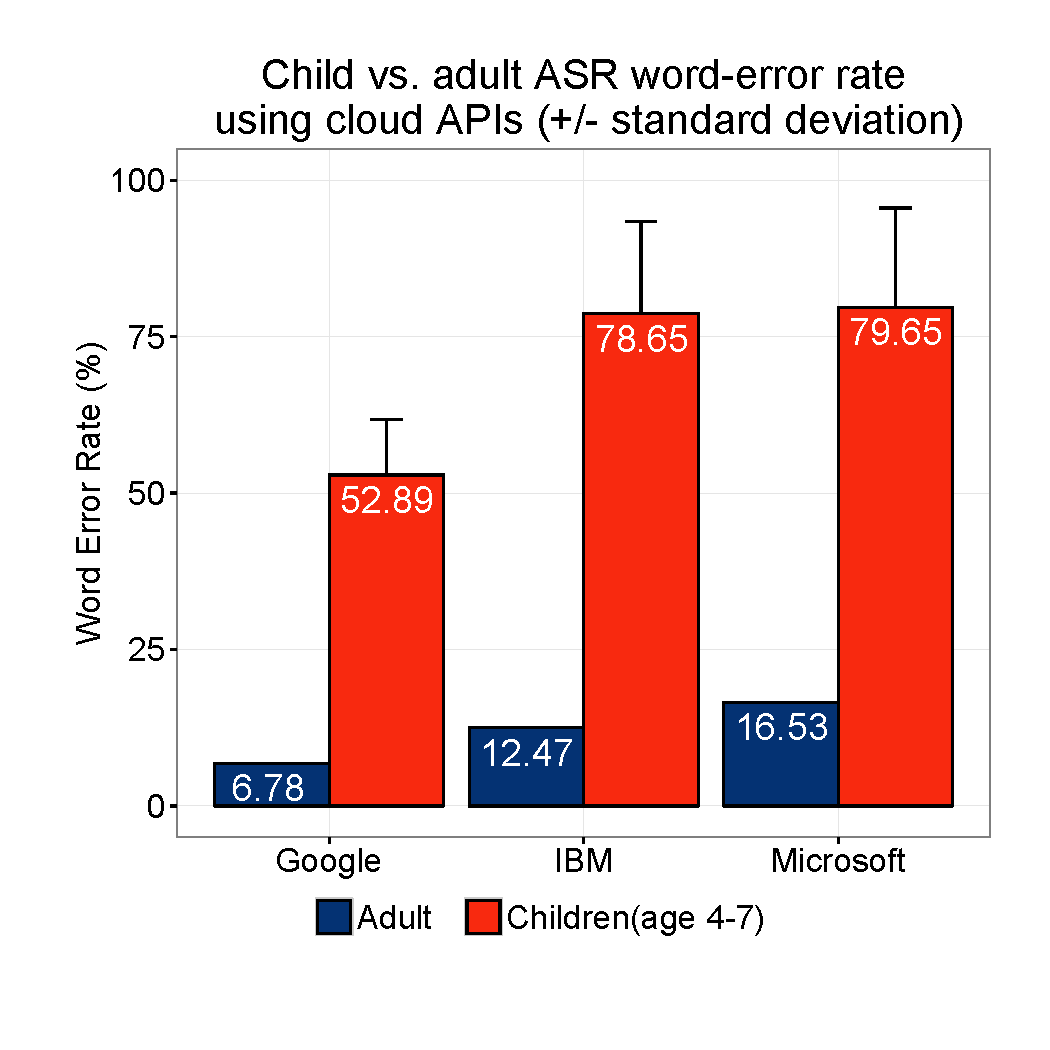
\includegraphics[width=0.35\textwidth]{fig/asr.pdf}  
 % \caption{The performance of the state-of-the-art ASR tools is far from functional on child speech.}
 % \label{fig:asr}
%\end{wrapfigure}

\subsection {Multi-modal automatic assessment algorithms for Kindergarten age children's spoken language and early reading skills}
\subsection {Automatic personalization algorithms for story content customization and dialogic question generation in the context of  young children's verbal storytelling}
\subsection {Development of a fully autonomous, collaborative, peer-like social robot system with effective educational activities that can do all the above.}
\subsection{Evaluation studies with deployed social robots in schools and homes demonstrating sustained engagement and positive learning outcomes.}


The ability to deliver effective, scalable, affordable, early literacy and language interventions to young children is a high impact area for the education system and parents. This proposed effort both integrates and expands our team's strong track record of foundational innovations in the development of social robot learning companion technologies that has yielded positive learning outcomes for young children in school deployments. We extend these efforts, and develop novel contributions, to develop a cloud-connected social robot learning companion system that can deliver an effective, socially situated, spoken language-oriented, and personalized learning experience for young learners focusing on early literacy and language learning.\\

\section{One Year Horizon of project}

We focus on reading and language skills as expressed during children's co-reading and story retell. Children enjoy telling stories, and while doing so they express their current level of language skills, (e.g., vocabulary, grammatical level, etc.) as well as their cognitive and social understanding~\cite{schank1990tell,wright1997creating}. Hence, analysis of children's stories within a theoretical-based framework can serve as an unobtrusive, continuous, and personalized assessment tool for a variety of skills. 

\section{Strength of Team to Achieve Proposed Milestones}

In light of the current research landscape at the intersection of social robots, early education, and spoken language understanding, we are in relatively unexplored territory, yet with the potential for high impact.  Our proposed work extends and builds upon our team's established track record of foundational research in the development of social robot learning companion and associated spoken interface technologies for children.

% Pics of robots would be good here
\pagebreak



%\begin{figure}[t]
%  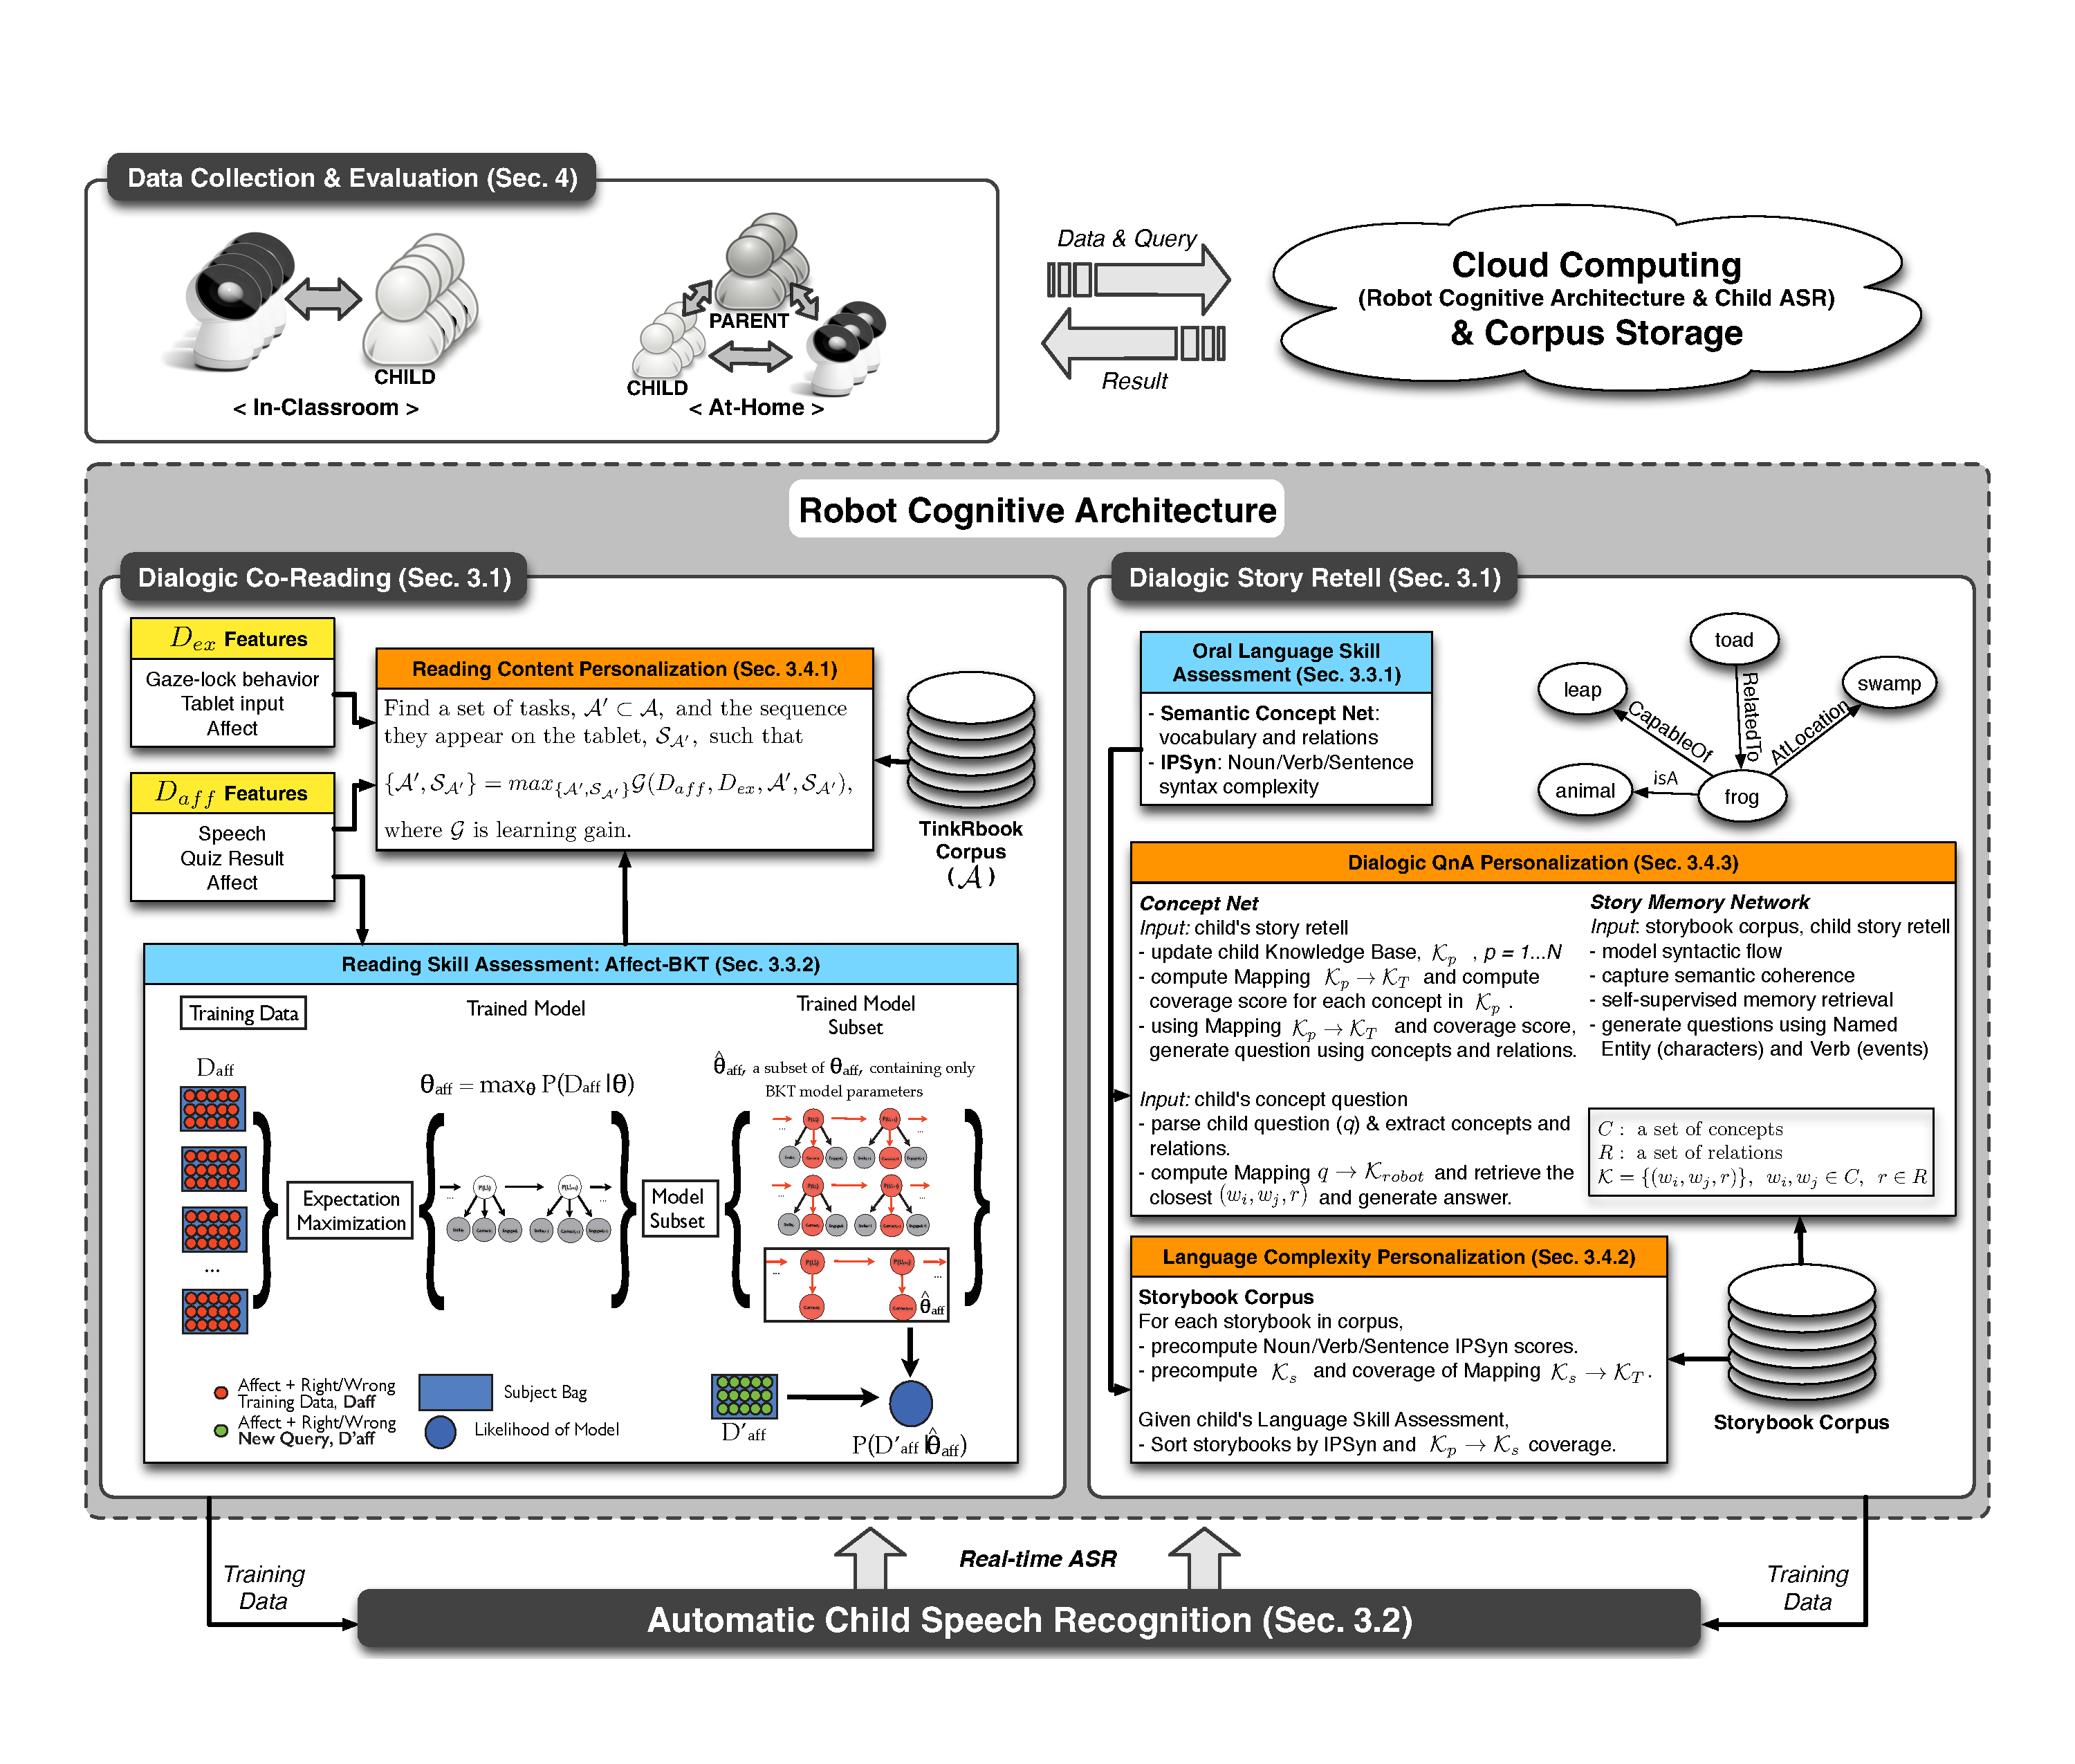
\includegraphics[width=\textwidth]{fig/NRI_arch.pdf}
%  \caption{Personalized Learning Companion Robot system components: Innovative Robot Cognitive Architecture and Child ASR shall be developed and implemented as part of the cloud computing platform, which during the interaction our robot will send queries and receive real-time results (Section~\ref{section_proposedwork}). Our system shall enable online assessment of kindergarten-age children's reading and spoken language skills, provide personalized content and interaction solutions, and adapt the robot's language and dialogic behavior to the child. We will develop data corpus and evaluate our fully autonomous, collaborative, peer-like social robot system through multiple pilot and longitudinal studies in classrooms and at homes (Section~\ref{section_evaluation}).}
%  \label{fig:system_arch}
%\end{figure}

Building on our prior works (see Section~\ref{section_priorwork}), we will develop two categories of educational activity apps that integrate automatic speech recognition (see Section~\ref{section_ASR}) and automatic assessment of reading and linguistic skills (see Section~\ref{section_assessment}), with personalized content adaptation (see Section~\ref{section_personalization}). These apps will be used to both capture children's speech and video  to train our proposed computational speech and assessment models, and to capture data to assess children's language and literacy outcomes from the social robot intervention.

The interaction scenario involves having the social robot ``play" educational activates with a child like a peer with a tablet as digital interactive storybook. The two primary activities are outlined below, and there will be a library of content  of grade-appropriate children's stories associated with each, and leveraging assets developed from prior work to support multiple-month deployments (see Section~\ref{section_ipsyn}).  From these activities, the social robot system shall capture real-time audio, video, touch interactions, and app states on the tablet. This data shall be uploaded and stored in our team servers (see Data Management Plan), where the team can access it to train our novel computational models, to assess children's reading and language performance, and to adapt these activities and the robot's behavior to each child to optimize motivation, engagement, and learning. 

{\bf Personalized, Dialogic Co-Reading:} where children are invited to ``tinker" with, to touch, or to read text from single words to short sequences of words along with the robot who demonstrates, prompts, encourages, and asks questions to support dialogic reading (see Section~\ref{section_storyretell}).  The interactive storybook design builds upon our prior research in developing innovative interactive storybook apps, called TinkRbooks, to foster early literacy and language skills~\cite{Chang_Breazeal_2011}.  As the activity progresses, our Affect-BKT assessment algorithm models the children's reading skill (see Section~\ref{section_SAR}). Meanwhile, the system personalizes the digital stories and robot's questions to prompt and motivate the child, to reinforce comprehension, and to advance through a curriculum that balances challenge with mastery to optimize engagement.

{\bf Personalized, Dialogic Story Retell:} where a child first listens to a story on a tablet then retells that story to the robot. The child's retell of the story is transcribed using our ASR model (see Section~\ref{section_ASR}), and the transcript is automatically analyzed for linguistic skill and complexity using our automatic IPSyn tool (see Section~\ref{section_ipsyn}). Based on this linguistic assessment, the robot's dialogic questions (see Section~\ref{section_dialogicquestion}), story content, and linguistic complexity of that content is personalized to the child during the session and in subsequent sessions according to the principles of Vygotsky's zone of proximal development (ZPD;~\cite{Vygotsky_1978}) which requires tailoring language just above a child's current level of capability. The level is achievable with assistance from an expert (in this case the social robot) fostering learning and sustained engagement. The robot then tells a different story to each child, personalized accordingly.

These activities can easily be adapted to support either in-school scenarios where a robot and child play these activities together or a triadic interaction in homes where a parent-child-robot do these activities together. In prior work with the TinkRBook, for instance, we explicitly did in-home studies to study the design impact of TinkRability on fostering parent participation during story co-reading. We were able to show that this new design principle encouraged  parents to perform a range of positive emergent literacy behaviors (print referencing, dialog, and dialogic questioning) by 3 to 10 times more than with reading physical books~\cite{Chang_Breazeal_Faridi_Roberts_Davenport_Lieberman_Montfort_2012}. Additionally, children were observed to take a more active role in exploring the concept of text. With social robot triadic interactions, we observe that parents participate naturally as part of the group and similarly help to guide, highlight, motivate, and prompt their child~\cite{Freed_2012}. These design principles will be incorporated and further explored in the proposed work.

\subsection{Automatic speech recognition for young children}\label{section_ASR}

Innovative Automatic Speech Recognition (ASR) and Spoken Language Understanding (SLU) technologies will be developed to assess and diagnose children's comprehension of early literacy and language material based on storytelling, co-reading, and answers to the robot's questions.The goals are to: 1) develop innovative ASR algorithms for young children that are robust to age, gender, classroom noise and disfluencies, 2) create innovative SLU algorithms to extract useful information from children's stories and answers to story-related questions, and 3) develop and validate diagnostic assessments that probe vocabulary and syntactic structure acquisition related to conceptual understanding.

Since unconstrained recognition of children's speech can be prohibitively challenging~\cite{fainberg2016improving}, we will constrain the domain to assessment of comprehension of early literacy and language materials. We focus on co-reading out loud, story retell, as well as answering dialogic questions about the stories because: 1)  For our targeted age group, speaking is the main mode of communication as they are at the earliest stages of learning how to read and write. 2)  A corpus of annotated speech from children's reading, retelling, or responding to questions from a known library of books constitutes crucially important research data to advance testing and teaching approaches, as well as the development of theories of cognitive strategies. 3)  Oral language can not only determine accuracy, but also provide clues to help diagnose understanding of vocabulary, word usage, confidence, and focus.  



Achieving the proposed goals presents several important challenges, including speech and language variability as a function of age, sex, socio-cultural factors, cognitive load, skills, and individual differences. Automated methods need to adapt robustly in the presence of such variability, while using information in the variability to discriminate among various learner states. Compared to adult speech, child speech is more challenging~\cite{price2009assessment,fainberg2016improving} due to (a) more omissions, substitutions, and mispronunciations, (b) shorter words that make discrimination more difficult, (c) more creative word use, (d) diversity in anatomy and physiology and developing motor skills, (e) larger variation in spectral and temporal parameters, and (f) larger number of disfluencies.  

The MIT team organized a workshop\footnote{IEEE RO-MAN 2016 Workshop on Enabling Long-Term Child-Robot Interaction: \url{http://web.media.mit.edu/~haewon/Roman-LTCRI/}} in 2016 to discuss the important enabling technologies for long-term child-robot interaction. The researchers elected child speech recognition as the top-most limiting factor in advancing child-robot research. The current state-of-the-art ASR models are mainly trained and evaluated on adult-speech corpora, such as the LDC\footnote{Linguistic Data Consortium: \url{https://catalog.ldc.upenn.edu/byproject}} training dataset. While various tools report achieving close to a single digit word-error rate (WER) on adult speech~\cite{saon2015ibm,xiong2016microsoft}, there is still no technology for child speech with accuracy rate above 50\%. Figure~\ref{fig:asr} shows our analysis of the performance of several cloud-based ASR APIs on child speech. We tested with a corpus of 5.5 hours of storytelling speech samples from 75 preschool and kindergarten children (ages 4--7 (5.13$\pm$0.64)), collected throughout our previous NSF projects. WER of an adult narrating a story used in prior studies is presented as a baseline for comparison. Overall, child-speech recognition rate was significantly lower than adult speech for all APIs (p < 0.0001), and their performance is unacceptable from a practical standpoint. An in-depth analyses of child speech ASR was recently published by Kennedy et al.~\cite{kennedy2017child}.

% \newcolumntype{S}{>{\centering\arraybackslash}m{1.5cm}}
% \newcolumntype{M}{>{\centering\arraybackslash}m{1.5cm}}
% \newcolumntype{L}{>{\centering\arraybackslash}m{1.8cm}}
% \begin{table}[h]
% \scriptsize
% \captionsetup{font=scriptsize}
% \resizebox{1.4\textwidth}{!}
% {\begin{minipage}{\textwidth}
% \begin{tabular}{S|S|S|S|S|S}
% Dataset (grade level) & \# of participants (female ratio) & Age (mean$\pm$sd) & Total \# of storytell sessions & Total sample length (hr:min:sec) & NSF grant\\
% \hline
% Dataset1 (Pre-K,K1) & 17 (0.59) & 4.88$\pm$0.49 & 177& 2:03:07&NSF CCF-1138986\\
% Dataset2 (K1,K2) & 40 (0.55) & 5.20±0.76 & 69 & 2:03:30 & NSF CCF-1138986\\
% Dataset3 (K2) & 18 (0.39) & 5.22±0.44 & 66& 1:25:22& NSF IIS-1523118 \\
% \hline
% Total & 75 (0.52) & 5.13±0.64 & 312 & 5:31:59 &\\
% \end{tabular}
% \caption[Table caption text]{Speech samples collected through storytelling activities at  different preschools and kindergartens.}
% \label{table:name}
% \end{minipage} }
% \end{table}


Most previous work on children's speech has focused on exemplar productions. We propose to focus on speech variants under co-reading and storytelling learning/assessment conditions. Understanding developmental changes in children's speech has helped us devise strategies for dealing with acoustic mismatch between different age groups and for designing robust ASR for assessment~\cite{alwan2007system}. We will investigate how speech and language cues emerge as learning develops by quantifying variation in segmental and suprasegmental properties (F0, duration) in a variety of learning and assessment scenarios. Understanding unconstrained spoken language is far from solved, but we envision progress towards this goal through 1) constraining and structuring the target application domain, and 2) using good prior models combining cue-based machine learning methods (exploiting lexical, prosodic and discourse information), and rule-based methods (within a pedagogically sound assessment framework).

In contrast to traditional unsupervised or fully-supervised adaptation, we will draw on datasets as needed for particular purposes. This will be particularly important for modeling the proposed populations, since children's use of language changes as they learn to tell more elaborate stories. We believe that the proposed techniques will generalize to other domains and result in novel speech modeling paradigms that go beyond the conventional ASR problem of phonetic transcription. Below we describe the tasks proposed including: Infrastructure (collecting additional data, adapting existing data structures and interfaces), Speech Processing (robustness to speaker and pronunciation variability, to noise, and to disfluencies), Modeling storytelling (assessing use of language, and student modeling), and Evaluation.

{\bf Infrastructure.} In addition to the acoustic model training, we will need data on what words children use in retelling stories and how they use them in order to train language models that will constrain the lexical search during recognition. For both the acoustic and language modeling uses, the data will be transcribed at the word level and annotated with the metadata (e.g., fluency ratings, correct/incorrect and other item ratings). (See Section~\ref{section_ipsyn} for our prior work in automatic crowdsourced transcription of children's stories).

{\bf Speech Processing.} Larger intra- and inter-speaker acoustic variability for children, relative to adults, requires that acoustic models account for larger acoustic parameter ranges and temporal and spectral variability. Dealing with environmental noises in the classroom is also essential for robust ASR. Disfluency associated with children's speech is another confounding factor as it creates complexity in acoustic modeling as well as in speech decoding using recognition grammars or language models. In order to address these major challenges, we will develop novel and robust conversational interfaces. To accommodate various assessments, we need to improve ASR accuracy and add new measures such as reaction times. Since our technology development relies critically on scaling up systems for a variety of children under several conditions, we suggest a phased iterative design approach. We will rely on mock-up design experimentation for the proposed assessment framework, especially in the initial stages, with transitioning interface design and automated analyses.

    
{\bf Robustness to Acoustic Variability.} Inter-speaker variations of acoustic characteristics of speech sounds constitute a major cause of performance degradation in ASR systems. Such variations are caused by differences in the vocal apparatus and speech motor control. To maintain ASR robustness against speaker variability and developmental changes, speaker adaptation and normalization techniques are applied to reduce spectral mismatch between training and testing utterances~\cite{leggetter1995maximum}. We propose to use subglottal-based normalization for rapid speaker adaptation~\cite{arsikere2014frequency}. In addition, we will apply constraints imposed by speech production theory to model speaker variability. The proposed techniques are transformative in that they will require short amounts of data (a few seconds) to perform adaptation utilizing articulatory constraints. 

{\bf Robustness to Background Acoustic Noise.} In addition to challenges related to the variability of children's speech, classrooms can be unfavorable environments for ASR because of the high degree and non-stationarity of background noise. Noise, for example, could arise from other speech-like signals (e.g., the cocktail-party effect) or from non-speech-like signals (e.g., air-conditioning noise). We will develop noise-robust ASR systems based on three approaches: noise-robust feature extraction, variable frame rate analysis, and missing feature theory.
    
The goal of ASR feature extraction is to design front-end features which retain discriminative information while suppressing information which may introduce confusability into the recognizer. In~\cite{strope1997model,strope1998robust} we offer successful front-end features, motivated by the human auditory system, which isolate and enhance spectral peaks. Another approach to noise-robust ASR, also motivated by human speech perception, is variable frame rate (VFR) analysis~\cite{zhu2003non,you2004entropy}. In VFR, features are sampled adaptively according to the discriminative importance of speech segments. In the proposed work, we will derive a channel-specific VFR framework, which will adaptively sample feature components differently based on the information present in various frequency channels. In addition, we developed noise-robust ASR utilizing missing feature (MF) theory. In MF-based systems, unreliable spectral components are located via mask estimation, and compensated for accordingly. There exist two types of MF approaches: data imputation and marginalization. Data imputation reconstructs unreliable spectrographic (time/frequency) data prior to recognition~\cite{borgstrom2009missing} whereas marginalization deemphasizes the effect of unreliable components during  recognition~\cite{cooke1997missing}. A major and challenging component of MF-based systems, however, is mask estimation~\cite{tan2014feature}. We will develop these noise-robust techniques and apply novel statistical model-based methods to derive improved reliability masks.

 	{\bf Robustness to Disfluency.} Disfluencies such as filled pauses, repetitions, false starts, hesitations and repairs are inherent in spontaneous speech interactions. Although disfluency detection is relatively easy when one has prior knowledge of the correct utterance (e.g., read speech), it has not yet been well addressed in spontaneous speech recognition. In the proposed work, we need to deal with spontaneous speech by dividing the problem of disfluency processing into two sub-problems: (1) disfluency detection in the input utterance and (2) disfluency assessment by post processing of the recognized utterance. The disfluency detection problem will initially deal with the creation of a recognition dictionary that includes lexical entries of disfluent sound objects such as partial words and non-speech sounds (e.g., lip-smacking, laughing, etc). Depending on how they were produced, these sound objects will be phonemically transcribed or entered as individual lexical objects using pre-defined transcription symbols. The transcribed data will be utilized for acoustic model training of disfluent sound objects.
    
{\bf Robustness to Pronunciation Variability.} In addition to acoustic modeling to reduce the effects of speaker variability, improved pronunciation modeling is also required due to large lexical pronunciation variability in young children (e.g.,~\cite{tepperman2006pronunciation}). Pronunciation variants of target words will be added to the recognition dictionary based on observed frequency in the training data. Such a multiple pronunciation dictionary can be augmented by applying hybrid pronunciation representations using variable length units (e.g., context-dependent phones, syllables, words) for better ASR performance. Once an optimal lexicon file has been derived for the domain, the multiple pronunciation dictionary can be used to realign the training speech data and train improved acoustic models. As more data are accumulated we will derive a rule-based system for generating possible pronunciation variants, based on age, in order to absorb some potentially unseen pronunciation variants and to enhance the multiple pronunciation dictionary.

Transformative results are expected from: a) pronunciation modeling and speaker adaptation techniques appropriate for children of various competency levels in English, b) child-specific language modeling including syntax, non- lexical events, and discourse phenomena as well as limited-domain natural-language processing for assessing comprehension, and c) novel noise-robust ASR algorithms.


\subsection{Automatic Assessment Algorithms}\label{section_assessment}

In our prior work, assessment of children's oral and reading skills were conducted offline, after children interact with a robot, which significantly hindered real-time robot behavior and curriculum personalization. This proposed work will enable online adaptation of these algorithms through innovative child ASR, collection of diverse corpus to train and improve affect knowledge models, and incorporating active learning methods to achieve real-time assessment and personalization.

\subsubsection{Oral Language Assessment}\label{section_languageassessment}
We shall build upon our prior work in developing IPSyn-based computational methods (Section~\ref{section_ipsyn}) for assessing children's oral language development while the interaction is happening. The robot will generate just-in-time dialogic questions based on this automatic assessment. For this proposed work, we shall also extend this system to investigate automatic ASR transcription using the story retell as a context to constrain the ASR models. We shall compare the performance of this automatic system to existing human crowdsourced transcriptions. 

\subsubsection{Reading Assessment}\label{section_readingassessment}

% \begin{wrapfigure}{r}{0.42\textwidth}
%   \centering
%   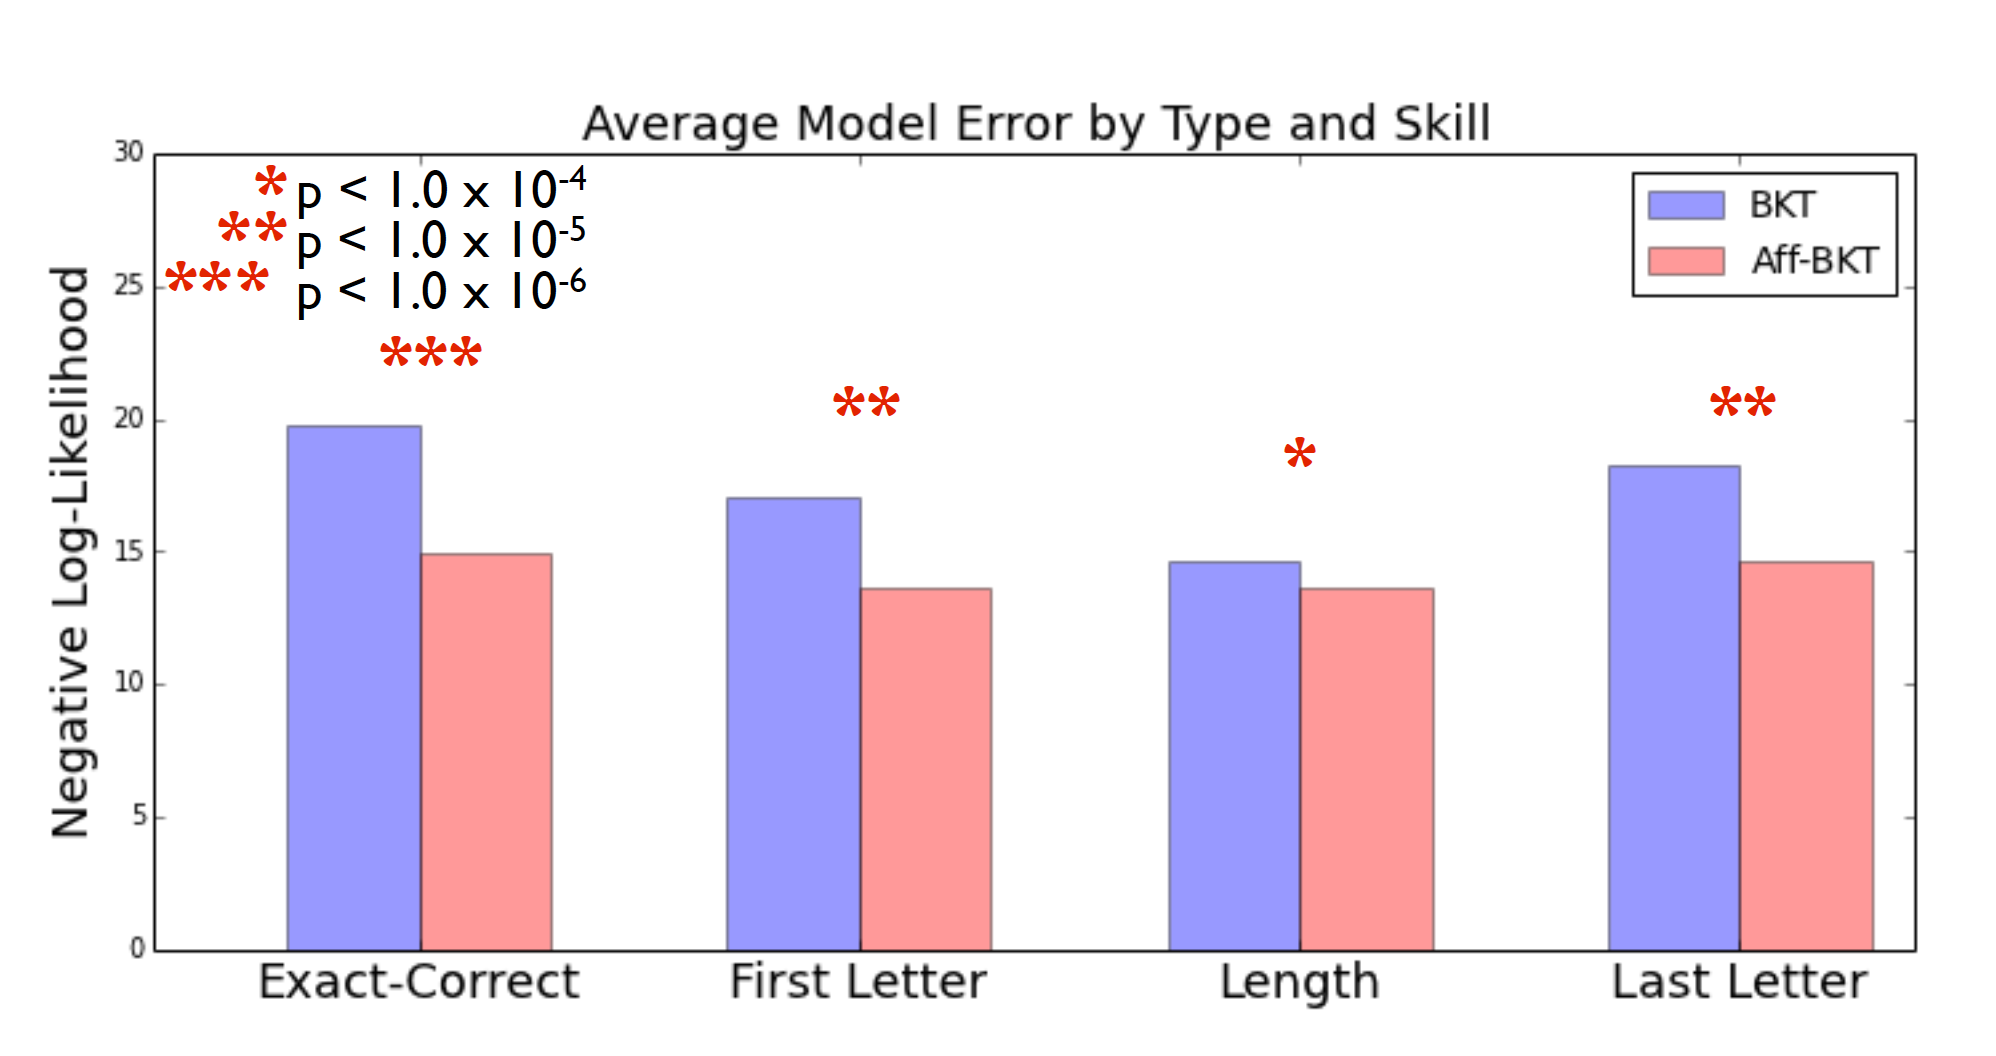
\includegraphics[width=0.4\textwidth]{fig/affect-bkt.png}  
%   \caption{Mean error estimates of BKT and Affect-BKT models by skill. Affect-BKT significantly decreases model error compared to traditional BKT.}
%   \label{fig:affectBKT}
% \end{wrapfigure}

Recall in our prior work (Section~\ref{section_SAR}), we showed that using affective information to create Affect-BKT model outperformed traditional BKT in assessing single-word reading skills~\cite{Spaulding_Gordon_Breazeal_2016}. 
%We focused on a single word reading task, modeling a set literacy skills known as ``alphabetic principle" skills~\cite{Byrne_Fielding-Barnsley_1989, Liberman_1989} to train four models, each corresponding to a word-reading skill (denoted as Exact-Correct, First-Letter, Length, and Last-Letter in Figure~\ref{fig:vocabulary}-(c)). 
Given our promising results with our Affect-BKT reading assessment algorithm  for young children, we propose the following extensions to develop a more advanced model that shall:

{\bf Span to Multi-word reading tasks.} Our previous work developed Affect-BKT models that more accurately assessed student's performance on foundational, one-word reading skills. We propose to extend these results to more advanced reading skills, e.g., assessing phrases and complete sentences.

{\bf Expand beyond tactile based inputs} {\bf to spoken inputs.} Our previous work relied on a child identifying (by tapping on a touchscreen) the written form of a spoken word to assess reading. More appropriately, though, reading is assessed by having the child speak a given word from its written form. The development of a robust child ASR model (Section~\ref{section_ASR}) will enable us to incorporate this more appropriate model of reading assessment into our methods.

{\bf Employ active-learning approaches} to improve algorithm convergence rate and accelerate model improvement. Generally speaking, Affect-BKT models improve with additional data. But collecting additional data often requires asking additional questions or prompting the child for new demonstrations of a skill. Maintaining child interest over a 20--30 minute educational interaction with an autonomous robot remains a challenge, which often limits the amount of useful data that can be collected in any single session. By employing an active-learning approach, we will ensure that the data we do collect provides the maximum expected inferential power, allowing the Affect-BKT models to accurately estimate a child's skill under real-world conditions and with practical data constraints.

{\bf Incorporate hierarchical and interdependent data structures} for skill inference. Previously, our models assumed that the alphabetic principle skills were mastered independently. Affect-BKT models are trained from the right/wrong quiz results and the affective QnA-interval data ($D_{aff}$) via expectation maximization, resulting in a set of learned model parameters, ${\theta}_{aff}=max_\theta P(D_{aff}|\theta)$ (see Figure~\ref{fig:system_arch}). We shall extend the Hidden Markov Model (HMM) structure of our previous Affect-BKT models to a Hierarchical Hidden Markov Model (HHMM) that captures the relationships and dependencies between skills and higher-order concepts essential to literacy development. 


{\bf Personalize to individual students.}  Our previous work developed Affect-BKT models trained on data from 38 children. By incorporating more diverse sources of real-time, real-world data as well as deploying the active-learning algorithms discussed above, we shall extend our work to develop personalized assessment algorithms, trained on a specific child's unique patterns of affective expression, attention, and prior knowledge.



\subsection{Personalization Algorithms}\label{section_personalization}

We shall iteratively develop a set of personalization algorithms based on human factors research and building on our prior work. Personalization algorithms shall incorporate both student performance data via assessments, as well as interpersonal cues such as affective data for valence, attention, and engagement, facial ID, and SLU analysis of prior recorded audio.

\subsubsection{Reading Content Personalization}\label{section_contentpersonalization.}
Based on a scope and sequence of target words and short word sequences per curriculum, our co-reading TinkRbook apps shall automatically adapt the challenge level of stimuli presented to the child. A child’s current skill, assessed by Affect-BKT using the child’s demonstrated skills (speech and app interaction) and affective states (a strong indication of confidence and engagement level), will be compared to the stimuli that are part of the curriculum scope and sequence. As part of our iterative human factors research in the first 3 years of the project, we shall develop an optimization algorithm for real-time adaptation of stimuli levels to maximize the child’s learning gain. Namely, inferring the combination of tasks with varying difficulty to effectively encourage and challenge each child, and deducing the sequence and location of how those tasks (individual apps) appear to children on a tablet. The difficulty of each task shall be expressed as a probability of learnability with the child’s current skill level, learning speed, and engagement as inputs to the function. Each child’s exploratory behavior will be used to develop an inference model to predict which app the child will select next, which will determine the tablet app placement strategy given a set of optimized tasks (see Figure~\ref{fig:system_arch}).   

\subsubsection{Oral Language Complexity Personalization}\label{section_storypersonalization}
The complexity of the stories during the story-retell task will be personalized to the currently assessed language skill of each child (i.e., their ZPD). Based on a scope and sequence within our specified story corpus (informed by co-PI Bailey and consultant Gottwald), we shall compute the linguistic complexity levels of each story according to their noun, verb, sentence complexity using the IPSyn score as a standard measure. Children's utterances will be similarly scored and assessed using the IPSyn tool by sentence type (fragments, questions, imperatives, complex, etc.).  Secondly, item-based patterns will be traced for their frequency. This process takes into account the growth of children's vocabulary knowledge and the relationships between their exposure to specific constructions and the occurrences of constructions in their own speech. We shall also compute a distance metric as a measure of the child's current demonstrated linguistic skill level relative to that of the stories in the corpus. The selection of a story for a given child is based on the (i) complexity level of synonymous adjectives, verbs, and nouns of each character and scene; (ii) complexity of the generated sentences to include specific syntactic constructions. While several automatic story-generation algorithms have been proposed in the past -- e.g., the Novel Writer system that generates murder stories within the context of a weekend party~\cite{klein1973automatic} to ground-up approaches leveraging non-deterministic simulations~\cite{leon2014creativity}, they have not addressed children stories, nor personalized content complexity. As part of our human factors research, we shall experiment with personalized story selection based on this distance metric, using engagement via facial expression as well as change in quality of children's story retell over time. 
 
\subsubsection{Personalized Dialogic QnA Generation}\label{section_dialogicquestion}
In prior work (Section~\ref{section_storyretell}), we were able to show the benefits of having a robot ask dialogic questions during a storytelling task. For example, %Figure~\ref{fig:dialogic} shows that 
children who responded to the robot's dialogic questions were more likely to use target vocabulary words and phrases in their story retell, and they tended to tell longer stories even after two months. These results suggest that the presence of dialogic questions helps children engage in the activity and focus their attention on specific elements of the story. 


While previous work used a pre-defined set of questions for all children, we shall develop automatic question generation algorithms for probing children's concept understanding and perspective taking. Dialogic questions will be generated in real-time and asked during and after a child's and robot's storytelling (see Figure~\ref{fig:system_arch}). More specifically, we focus on developing the following: \textbf{Story Memory Network:} Our robot storyteller shall automatically generate story-context questions for the stories in our corpus. First, we will track story's characters/scenes (named entities) and events (verbs) through explicit memory representation. Using memory network, we shall model syntactic flow of the story, detect semantic coherence, and develop word-level and sentence-level memory representation using {\it window memories}~\cite{hill2015goldilocks}. In addition to asking questions during its storytelling, the robot will, as part of its backchannel (listener response) feedback, prompt children with questions while they are telling a story. These questions will be more open-ended since tracking a story plot and asking questions at the right timing is difficult in real-world interaction (the rule-of-thumb is, any listener feedback should happen within 500ms of detecting backchannel opportunity~\cite{park2017hri-bc}). Hence, we will use shorter {\it window memories} and generate questions probing for character's internal landscape and change of perspectives (example: ``How did the boy feel when the frog was gone?"). The objective is to prompt and encourage children to think about the perspectives of the characters and the events that occur around them and incorporating them into a story narrative. 

Through longitudinal studies, we shall study whether children answering dialogic concept/story questions has long-term effect in language learning as well as engagement. For evaluating a child's concept growth, we will define a coverage score from the mapping $Map: \mathcal{K}_p \rightarrow \mathcal{K}_T$. Furthermore, all participants' $\mathcal{K}_p$ combined, we shall gain some insights into kindergarten children's general semantic network growth.

% Previous Work
While speech recognition technology has improved dramatically in recent years, an adequate tool for children's real-time speech recognition is not available. Our approach has been to circumvent this issue by recording children's stories and automatically sending these recordings to crowdsourced mechanical turk transcription services. We have successfully evaluated this oral language assessment tool on a corpus of children's storytelling speech data (hand coded by IPSyn score experts) with an accuracy of 94\%, as well as on a public CHILDES (Child Language Data Exchange System) dataset~\cite{macwhinney2000childes} with an accuracy of 91\%. (Publications in process). While very flexible and robust in output transcription, the downside is that the robot does not understand and cannot assess the child's current spoken story, but only prior stories told in the previous sessions.

%\required{Broader Impacts}
% As in the project summary, broader impacts of the proposed work
% must be called out separately in the project description.  
% You may be able to give more specific examples, 
% or discuss how you've previously achieved these impacts.
% It should be similar, but not identical, to the Broader Impacts statement
% in the project summary.

\section{Results From Prior NSF Support}\label{section_priorwork}
% Must be fewer than 5 pages of the entire description document of 15 pages.
% This section refers to any prior or current  NSF funding support
% with a start date in the past five years.
% If you have no prior support, it is still recommended to include this
% section and just indicate "The PI has not previously been supported by the NSF".
%If you have more than one award, you need only report on the one award most
% closely related to this proposal.
% The following information must be provided in this section:
% (a) the NSF award number; amount and period of support
% (b) the title of the project
% (c) a summary of the results of the completed work, including
% accomplishments, supported by the award. 
% The results must be separately described under two distinct headings, 

% TODO "see facilities section" above needs ref!


% \begin{figure}[tbp]
%   \centering
%   \subfigure{
%   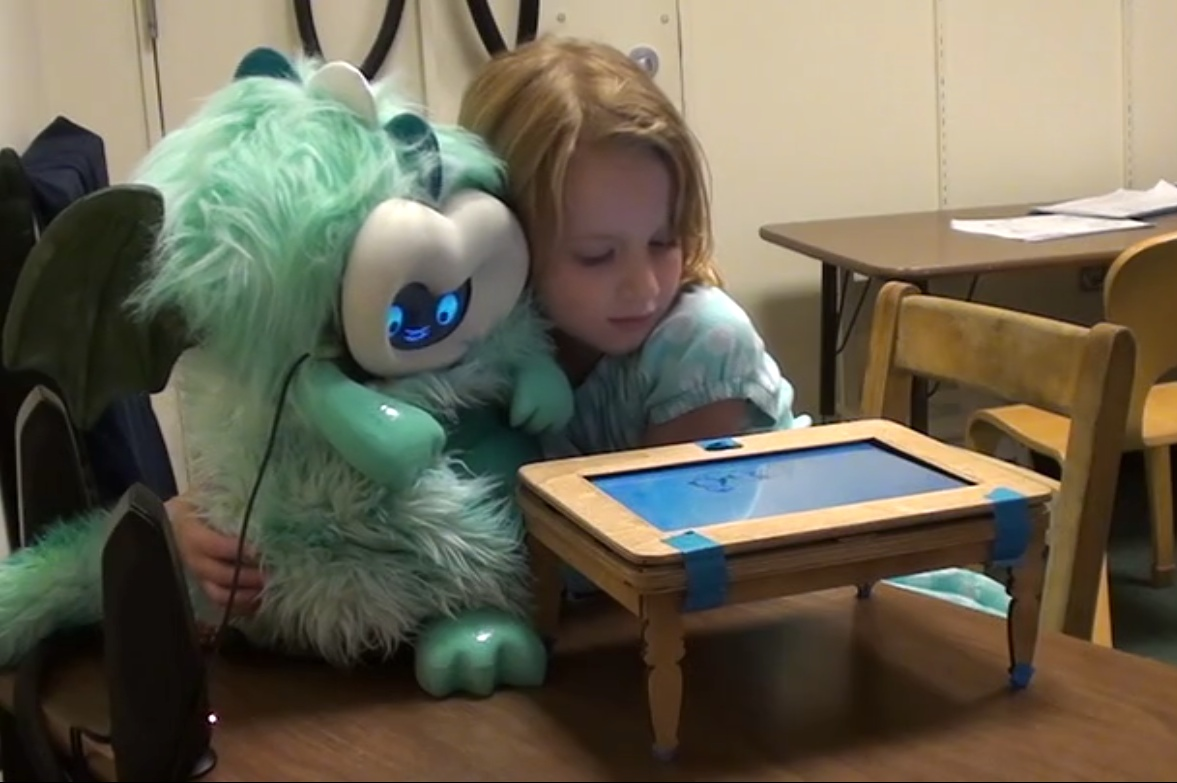
\includegraphics[height=0.15\textheight]{fig/Personal-Robots.jpg}}
%   \subfigure{
%   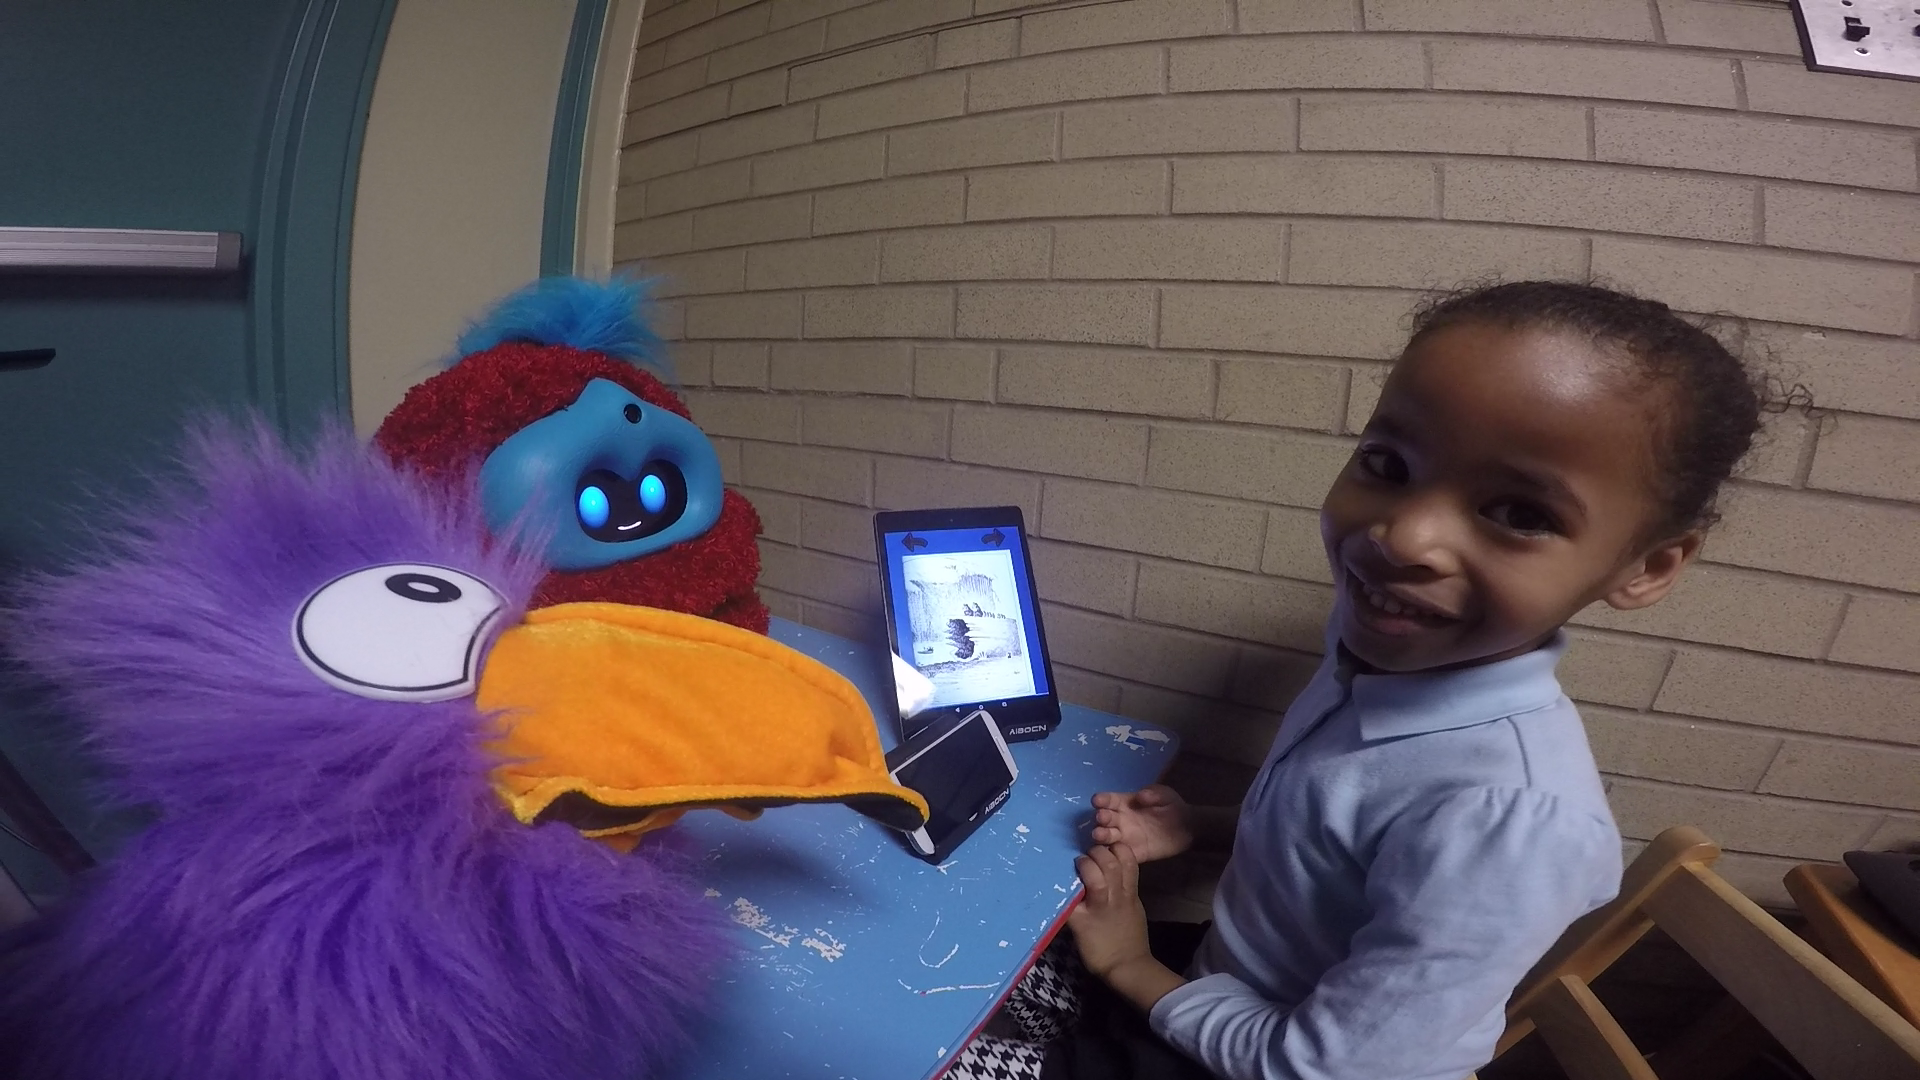
\includegraphics[height=0.15\textheight]{fig/cyber4-expressivity-2.png}}
%   \caption{Two social robot learning companion platforms with tablet as interactive digital storybook. Dragonbot in preschool classroom (left). Tega in story retell task with Kindergarten classroom (right).}
%   \label{fig:tega}
% \end{figure}
% * <cynthiab@media.mit.edu> 2017-01-24T12:02:02.321Z:
% 
% I put these images in the Facilities section so we can refer to them there. Saves space.
% 
% ^.
Personalization in the form of leveling the complexity of the story the robot tells to the child can therefore not happen during a session, but only in later sessions. To personalize the level of the story the robot tells to the child, we ran our language analysis tool on transcriptions of over 30 children's stories to calculate each IPSyn score. Experts then leveled the complexity of each story to create 3 variants, each having a different level IPSyn score. This represents a significant library of robot story assets that can span several months.  Based on the IPSYn score of the child's oral language in the prior storytelling session, the robot selects a story of a similar (if not slightly higher) IPSyn score.

{\bf Risk Mitigation and Proposed Extensions.} This prior work substantially mitigates risk in the development of an automatic oral language assessment tool in this proposed work. But it is not real time. The primary advance we want to make in this Project is to integrate the proposed automatic speech recognition technology to add real-time speech analysis, albeit in a more constrained scenario. While many advanced automatic speech recognition (ASR) tools now achieve more than 90\% accuracy with adult speech, the state-of-the-art for child ASR is far from functional - only achieving at most 50\% accuracy per our evaluation of cloud-based APIs. (See Section~\ref{section_ASR}) Furthermore, while natural language processing has advanced tremendously in recent years, especially in story understanding~\cite{graesser2004coh,nye2014autotutor}, a developmental theory-based approach for automatically analyzing children's spoken stories has yet to be addressed. In addition, the story content library developed as part of this prior work mitigates the risk of having insufficient story content for the social robot to engage children over a several-month long study.

\subsection{DIP: Collaborative Research: Social Robots as Mechanisms for Language Instruction, Interaction, and Evaluation in Preschool Children}\label{section_storyretell} 
\vspace{-0.5mm}\hspace{8mm} {\it NSF Cyberlearning IIS-1122886 \$387,993 (09/2011 - 08/2015)} Breazeal (co-PI), Park\vspace{2.5mm}

{\bf Broader Impact.} The goals of this work were to determine the extent to which various non-verbal expressive characteristics are necessary for a social robot to effectively engage young children in early literacy learning activities, and second, whether such a robot could be effective at engaging both native English speaking children and English Language Learners (ELL). 

{\bf Intellectual Merit.} As part of this larger goal, we investigated whether an expressive social robot could engage preschool and Kindergarten children in dialogic book reading (where the robot asks the child questions during storytelling). Prior research has shown this is an effective method for expanding young children's vocabulary. Furthermore, given the established effectiveness of dialogic reading, we also asked whether the robot's effectiveness was critically dependent on the expressive characteristics of the robot. 

A total of 45 children participated in the study. Each child first heard a story told by the social robot using a tablet as a digital picture book (in either an expressive or neutral condition). The robot asked the child a set of pre-determined questions during its telling of the story. The child was then asked to retell that same story, using the digital picture book if desired, to a puppet who missed the first telling. Children's oral language and non-verbal behaviors were analyzed to evaluate the impact of the robot's expressivity on children's overall retention of the story, oral language phrasing, and vocabulary acquisition. 

Our results (under review) show that the variation in the robot's behavior had a detectable effect on children's story processing. Both the native English speaking children and the ELL and bilingual children showed more engagement and concentration in the Expressive condition as indexed by their facial expressions. They emulated the robot's story more in their story retells, showing peer-to-peer modeling of the robot's language (i.e., using phrases and words that the robot had used). These children more frequently included the newly acquired vocabulary words in their retells, and they also recalled the story better during their delayed retelling. Furthermore, the more often children answered the robot's dialogic questions about the story, we found 1) greater phrase emulation in their story retells, 2) greater likelihood to correctly identify target vocabulary words, 3) greater use of  target words in their story retell, and 4) improved recall and retention of more information in the robot's story even after a 2 month delay (Figures).  These results also highlight the importance of designing robots as social agents, with social and expressive characteristics, to garner the greatest benefit to children's language learning.

{\bf Risk Mitigation and Proposed Extensions.} This prior work substantially mitigates risk around children's engagement and ability for children's oral-language behavior to benefit from a dialogic storytelling task with story retell. It also validates the appeal and value of an expressive social robot on children's performance. As a result, we use this core collaborative interaction paradigm and activity in this Project. A key extension is to integrate ASR and spoken language understanding so that the robot is able to generate personalized questions to the child during dialogic storytelling and retell (see Section~\ref{section_dialogicquestion}).

% \begin{figure}[tbp]
%   \centering
%   \subfigure[]{
%   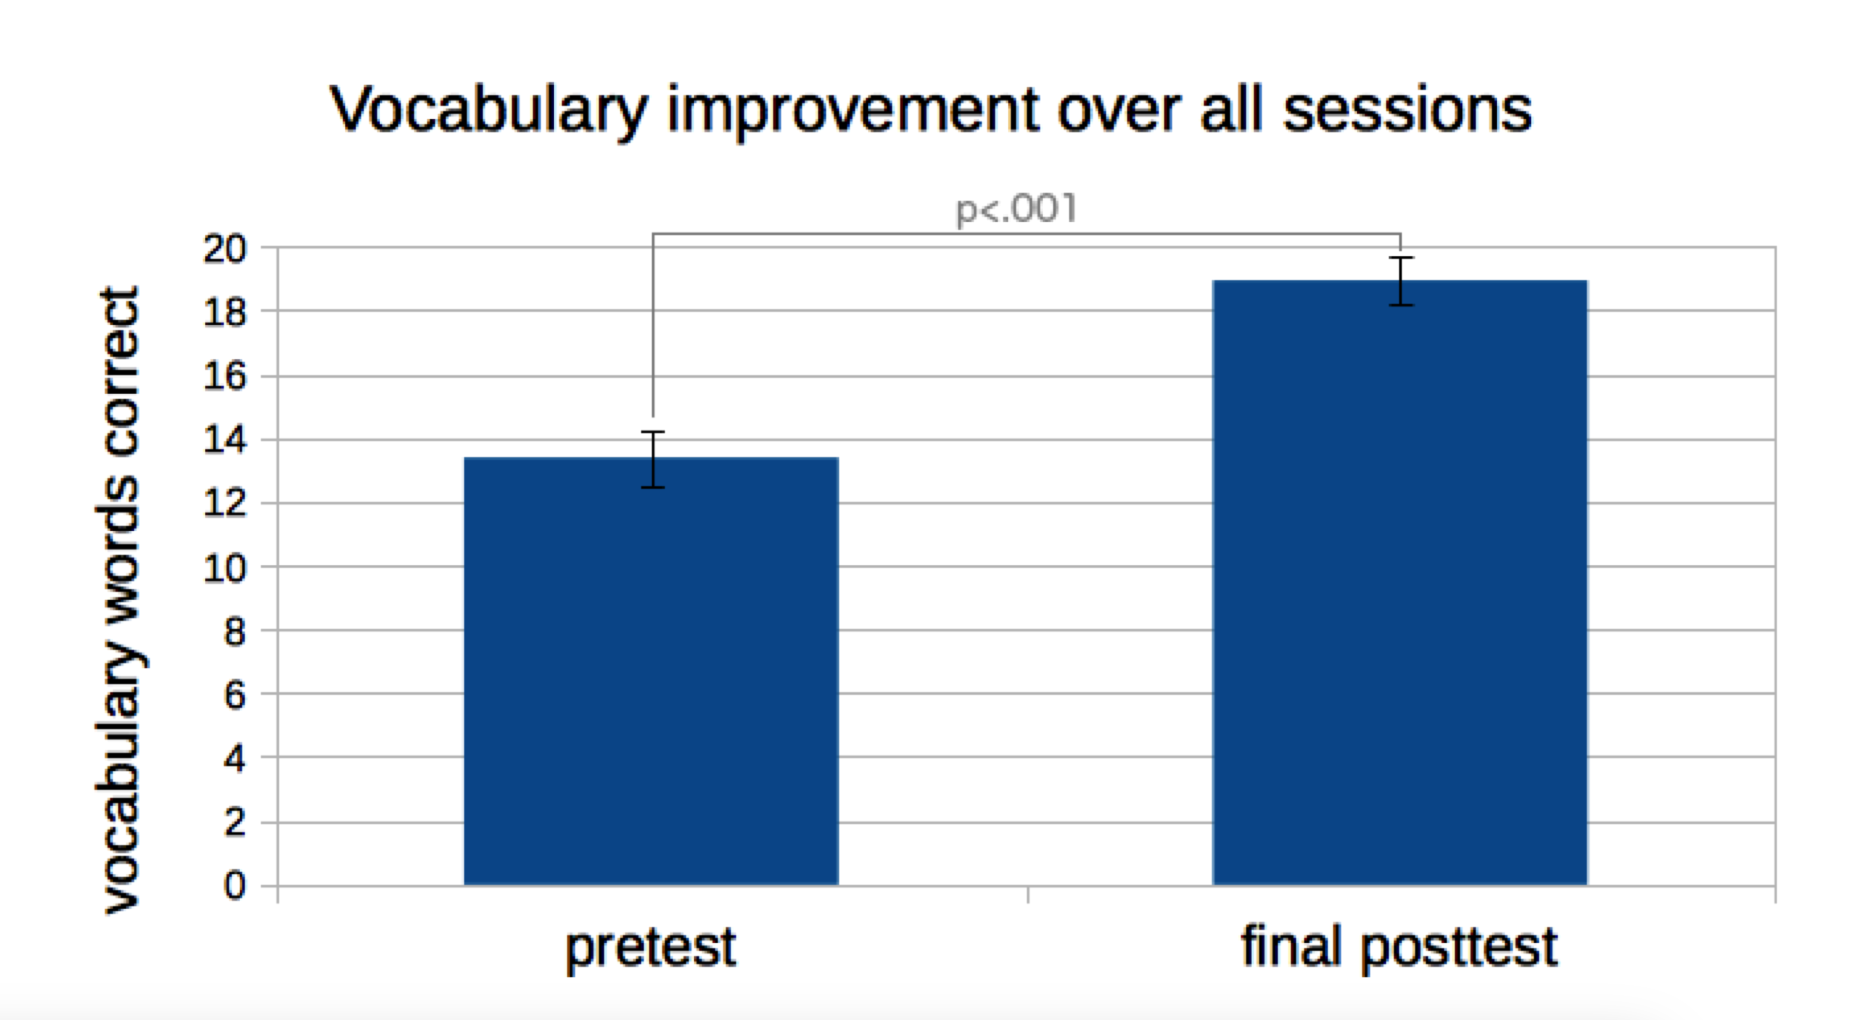
\includegraphics[width=0.3\textwidth]{fig/Vocab-pre_post.png}}
%   \subfigure[]{
%   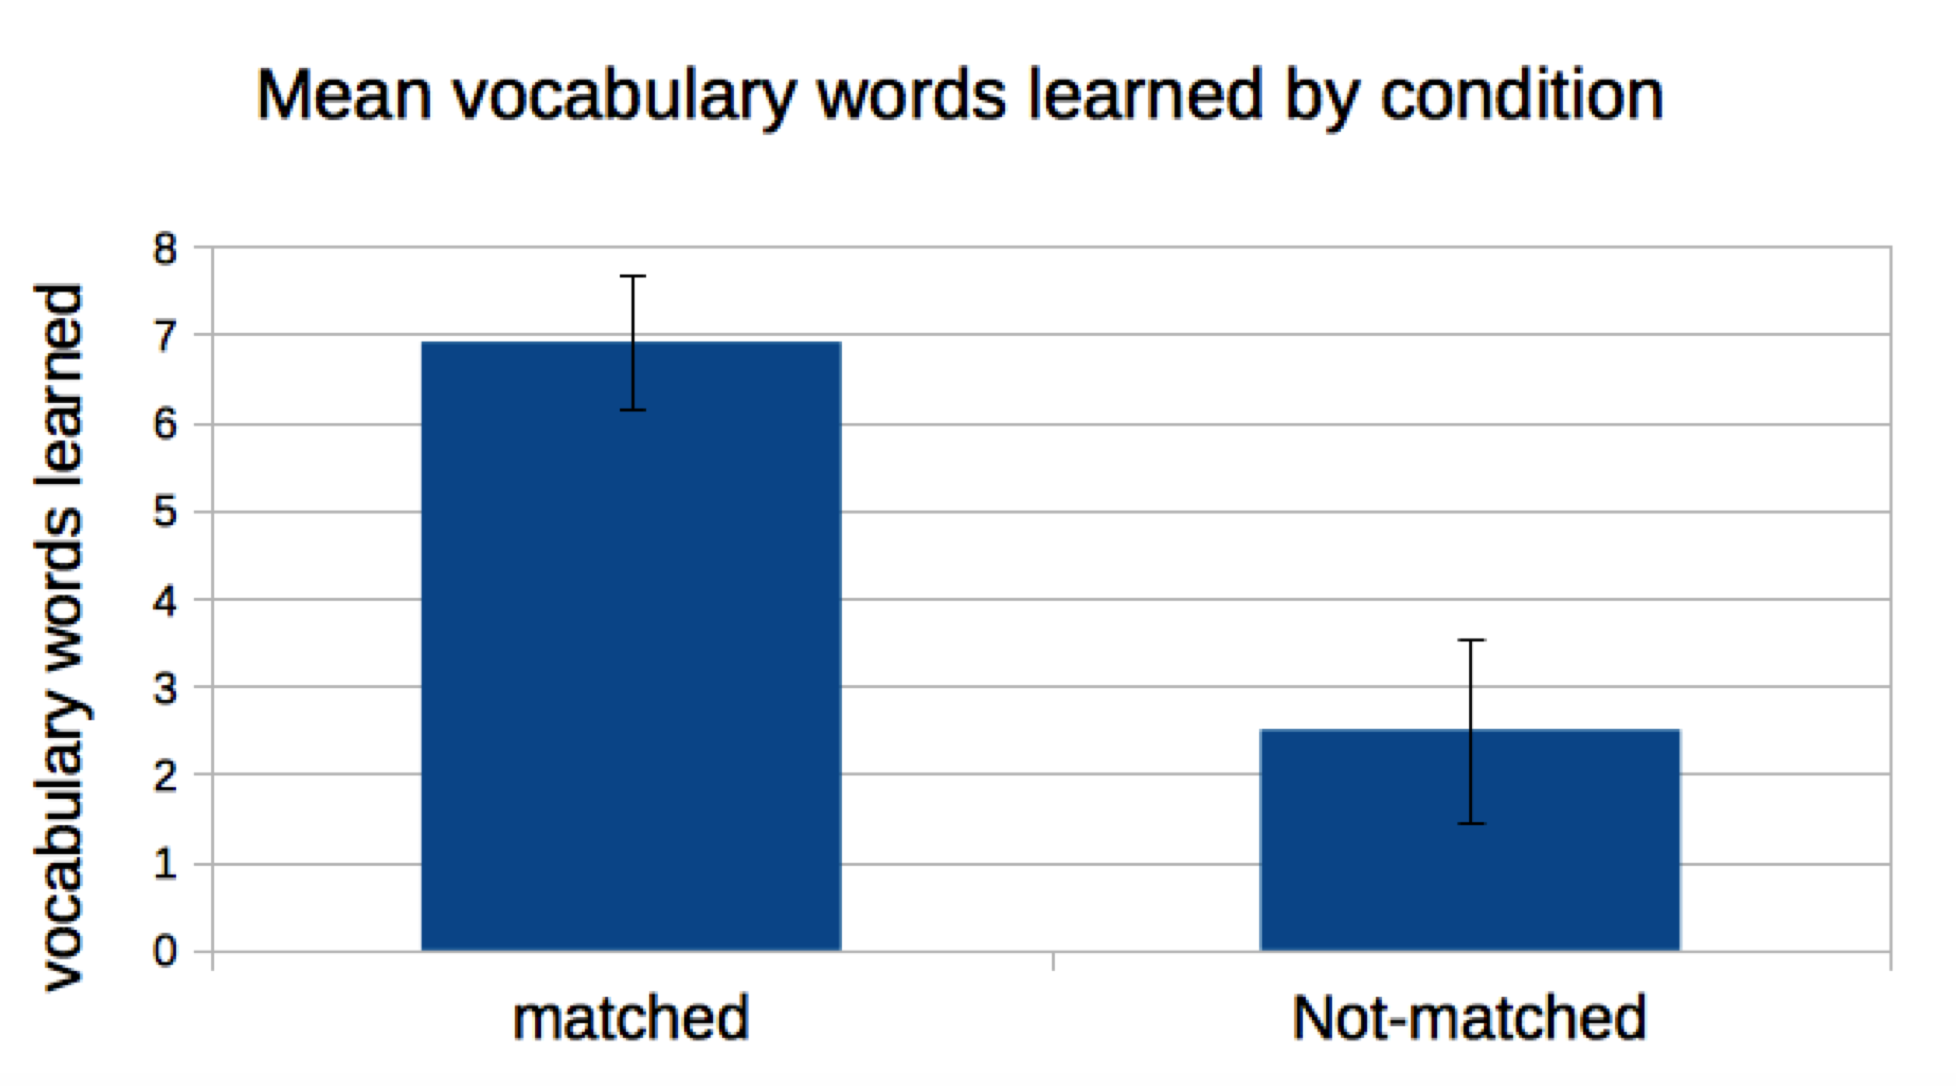
\includegraphics[width=0.29\textwidth]{fig/vocab-matched_notmatches.png}}
%   \subfigure[]{
%   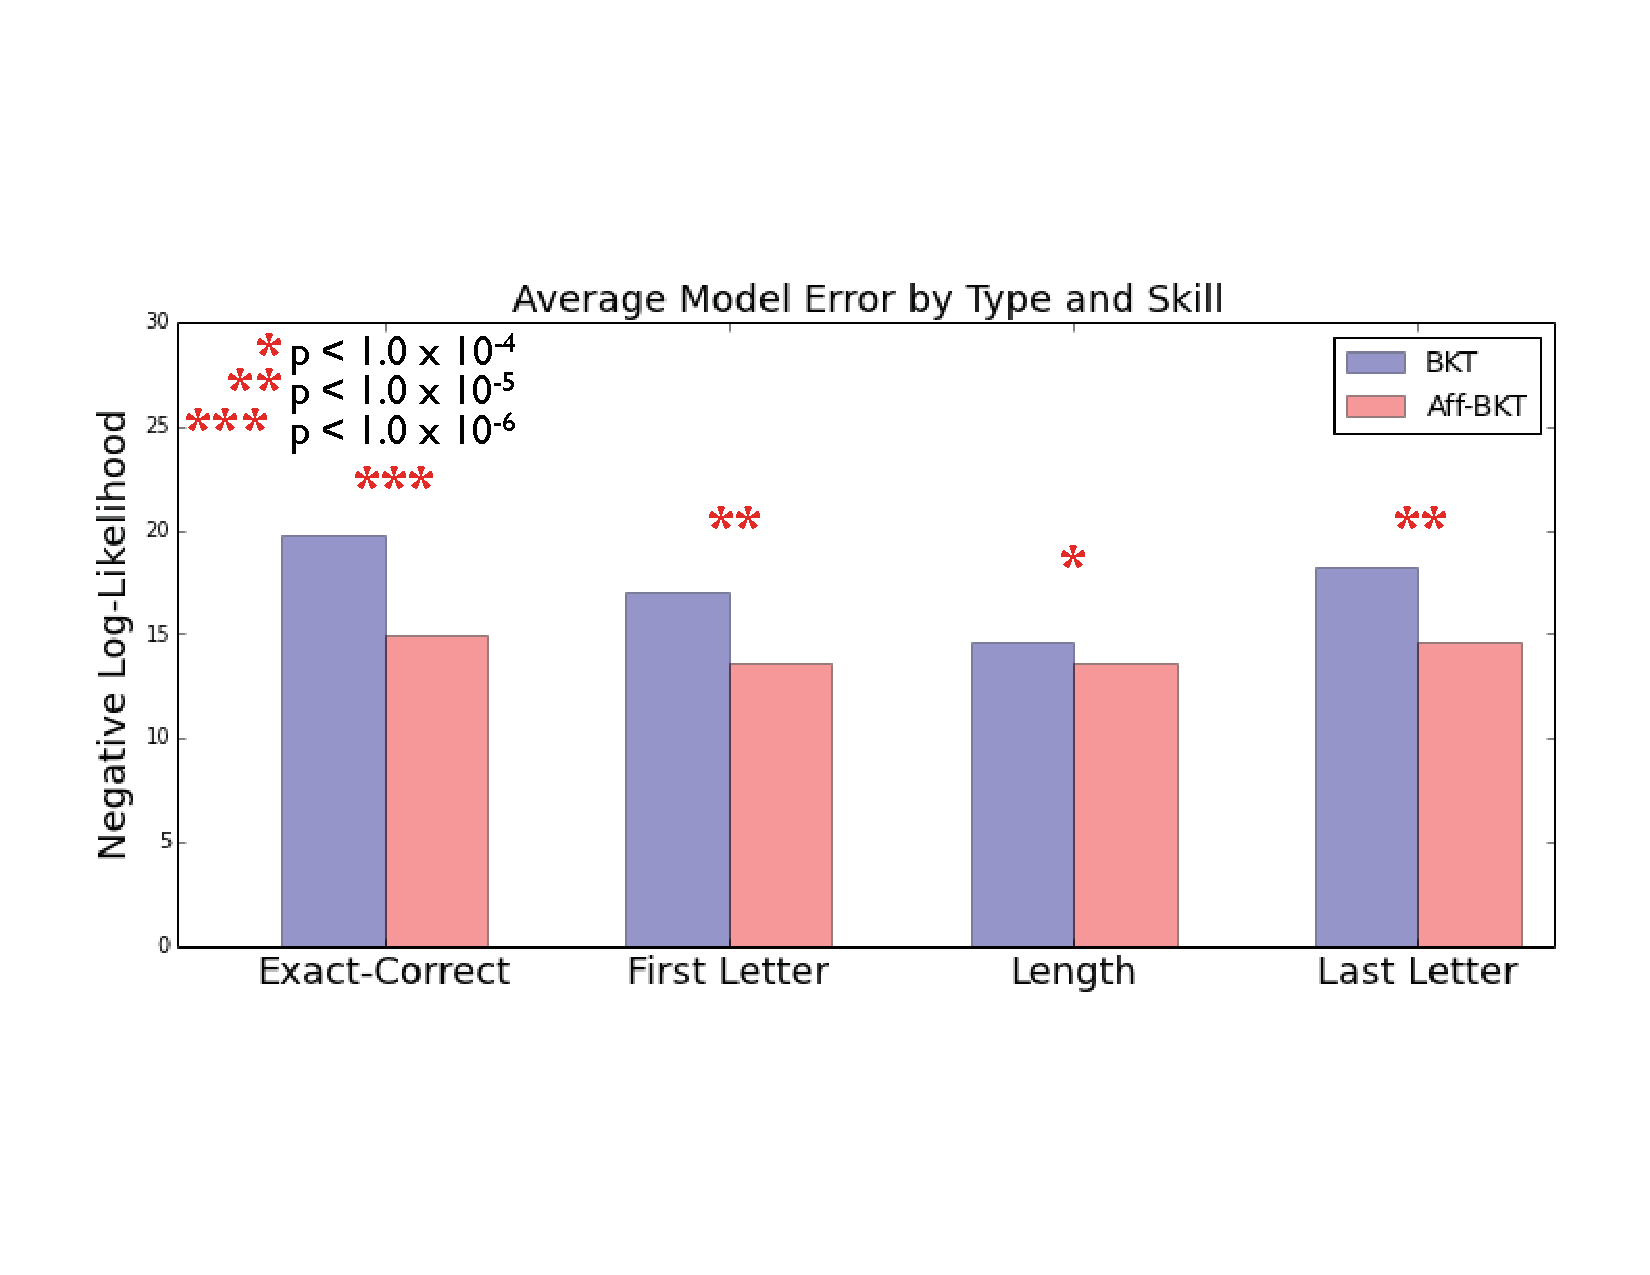
\includegraphics[width=0.36\textwidth]{fig/affBKT-result.pdf}}  
% %   \caption{The performance of the state-of-the-art ASR tools is far from functional on child speech.}
%   \caption{(a) Children successfully learned new words from the story sharing task with the robot across all conditions. (b) Children learned more vocabulary words when the robot matched the child's language level. (c) Mean error estimates of BKT and Affect-BKT models by skill. Affect-BKT significantly decreases model error compared to traditional BKT.}
%   \label{fig:vocabulary}
% \end{figure}

% \begin{wrapfigure}{R}{0.4\textwidth}
%   \centering
%   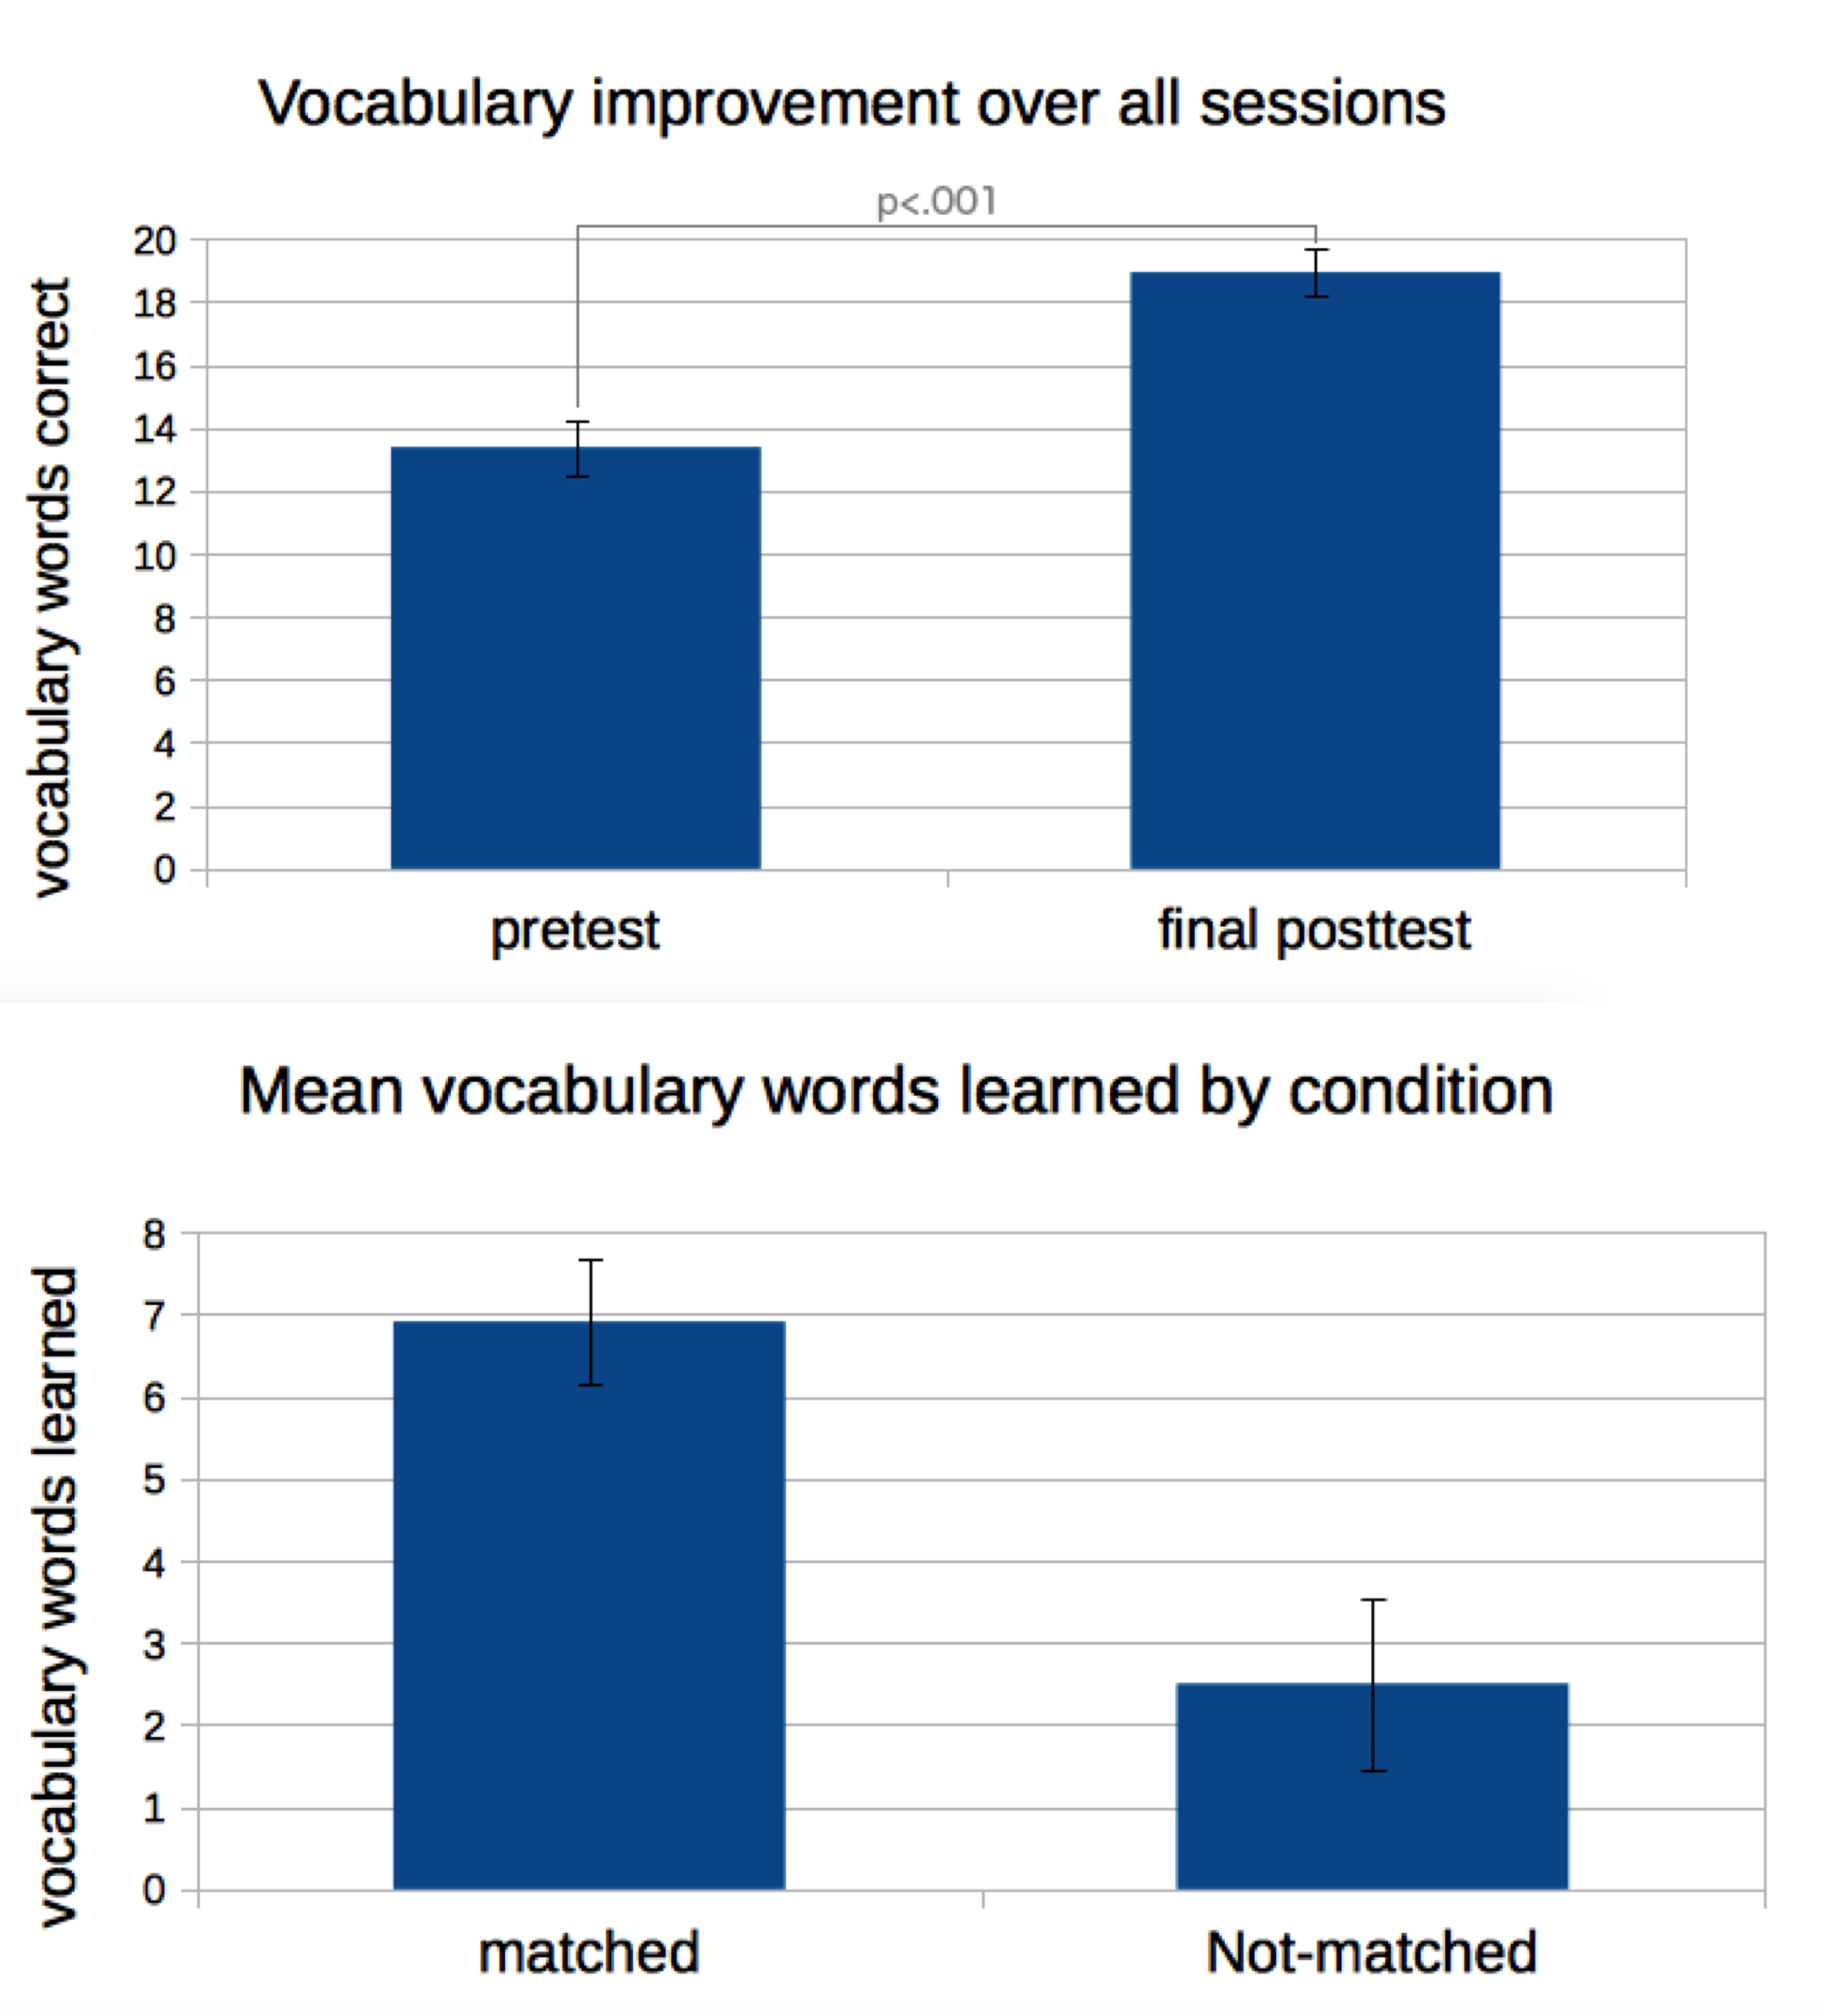
\includegraphics[width=0.35\textwidth]{fig/vocab.png}
%   \caption{(Top) Children successfully learned new words from the story sharing task with the robot across all conditions. (Bottom) Children learned more vocabulary words when the robot matched the child's language level.}
%   \label{fig:vocabulary}
% \end{wrapfigure}

\subsection{DIP: Collaborative Research: Socially Assistive Robots}\label{section_SAR}
\vspace{-0.5mm}\hspace{8mm} {\it NSF CISE Expeditions in Computing CCF-1138986 \$2,075,000  (04/2012 - 03/2017)} Breazeal (co-PI)\vspace{2.5mm}

{\bf Broader Impact.} The primary goal of this Expedition is to develop socially interactive robots that can serve as a long-term, personalized social companion for children in three domains: health adherence, education with focus on language learning, and autism spectrum disorder.  


{\bf Intellectual Merit.} A key question that predicates this Project is whether a social robot, modeled as a peer, can facilitate preschool children's oral language and vocabulary development over a longitudinal story sharing intervention. We focused on the personalization of the robot's language complexity during a storytelling game and its potential impact on children's own storytelling or ability to learn new words from these stories. A total of 17 preschool and kindergarten children were divided into level-matched and level-unmatched groups and played a storytelling game with a tele-operated robot for 8 sessions over a period of 2 months. In the ``matched" condition, the robot told a story that was selected to match children's pre-assessed language ability. In the ``unmatched" condition, the robot had a fixed agenda of stories that did not consider the pre-assessment results. Our results show that children can successfully learn new words from a robot storytelling companion over repeated encounters, and children indeed learn more words when exposed to a level-matched story complexity (p<.001). Furthermore, children's level of engagement and entertainment during this discourse remained high, and we saw increasing peer-like interactions over time~\cite{kory2014storytelling,Kory_Breazeal_2014}. 

Building on this early result, we began to advance the autonomy of the robot. We developed an early literacy assessment algorithm to estimate young children's reading skills and knowledge. We developed an innovative, affective variant of the Bayesian Knowledge Tracing (BKT) model, Affect-BKT. Affect-BKT is trained with students' affective expressions, such as frustration, discomfort, and engagement measured by the Affectiva\footnote{Affectiva \& Affdex SDK -- a commercial, FACS-based affect-analysis tool trained on data from over 2.7 million faces in 75 countries~\cite{swinton2012measuring,mcduff2012affectaura}.} software, in combination with students' performance data as contextual information to infer their comprehension level of a given task. We evaluated Affect-BKT with single-word reading tasks, modeling a set literacy skills known as ``alphabetic principle" skills~\cite{Byrne_Fielding-Barnsley_1989, Liberman_1989} to train four models, each corresponding to a word-reading skill (denoted as Exact-Correct, First-Letter, Length, and Last-Letter). The Affect-BKT knowledge inference model outperformed traditional BKT in all four reading skill assessments~\cite{Spaulding_Gordon_Breazeal_2016}. 

{\bf Risk Mitigation and Proposed Extensions.} Our pilot storytelling study mitigates risk around young children's ability to learn vocabulary from a social robot modeled as a peer in a storytelling context. It also mitigates risk that children can stay engaged over several weekly sessions, and that repeated exposure over 8-weeks is sufficient to see vocabulary gains (but we did not see broader language gains such as syntax complexity). We also observed that adapting the complexity of the robot's language to children's level improves learning outcomes, albeit the personalization was fairly coarse and un-nuanced. Also, every aspect of the robot was teleoperated. Nonetheless, this proof-of-concept sets a compelling stage for autonomous social robot learning companions, capable of greater personalization and social engagement, for early language and literacy development. In our subsequent reading task work, we mitigate risk around young children's ability to engage in a co-reading task with a robot, and our ability to develop basic reading assessments focusing on alphabetic principles (appropriate for Kindergarten age children). In this work, we also validated the potential usefulness of using affect to assess children's skills with greater accuracy. As a result, we will use this co-reading paradigm as one of our core activities. See Section~\ref{section_readingassessment} on proposed extensions to move this work beyond a proof of concept to a fieldable assessment. 

\subsection{IERI Collaborative Research: Automating Early Assessment of Academic Standards for Very Young Native and Non-Native Speakers of American English} 
\vspace{-0.5mm}\hspace{8mm} {\it TBALL ITR/IERI 0326214 \$2,270,000 (9/2003-8/2008)} Alwan (PI) and Bailey\vspace{2.5mm}

{\bf Broader Impact.} The project supported 12 Ph.D., 4 M.S., and 10 undergraduate students in EE, CS, and Education, 2 Postdocs, 6 K-5 teachers, and a high-school student. It resulted in more than 29 publications and presentations, and a book. 

{\bf Intellectual Merit.} The project resulted in a battery of assessments guided by specific goals to inform instruction. Specifically, we developed a framework for assessing basic reading skills for children in grades K-2 using a hierarchical, drill-down approach, automated some of the assessments using automatic speech recognition (ASR) and techniques to measure rate and fluency, developed interfaces for both children and teachers, developed a query-based data-mining system, and provided guidance to teachers on the use of appropriate assessments to monitor progress and assist with diagnosis. Assessments targeted skills including phonological awareness, alphabet-to-sound mapping, word decoding, sight reading of familiar and nonsense words, fluency, and domain-specific comprehension. ASR capabilities can automate scoring of isolated words and sentences from ELL and non-ELL children with high accuracy. 

\subsection{EAGER: Collaborative: Models of Child Speech}
\vspace{-0.5mm}\hspace{8mm} {\it NSF CISE RI-1551113 \$140,000 (7/2015-2/2018)} Alwan (PI)\vspace{2.5mm}

{\bf Broader Impact.} The project contributes to the knowledge of variability between children, as well as variability over time as children grow. It will significantly advance knowledge of speech production development and its relationship to machine recognition of children's speech. The work provided partial support to 2 PhD, 2 MS students, and 2 undergraduate students in Engineering and Linguistics, and produced 5 publications. 

{\bf Intellectual Merit.} The project reveals processes of speech production development in elementary school-aged children through a unique combination of articulatory and acoustic analyses. 

\section{Proposed Work}\label{section_proposedwork}

\subsection{Reading and Storytelling Activities for Curriculum and Data Capture}\label{section_activities}

We focus on reading and language skills as expressed during children's co-reading and story retell. Children enjoy telling stories, and while doing so they express their current level of language skills, (e.g., vocabulary, grammatical level, etc.) as well as their cognitive and social understanding~\cite{schank1990tell,wright1997creating}. Hence, analysis of children's stories within a theoretical-based framework can serve as an unobtrusive, continuous, and personalized assessment tool for a variety of skills. 

\begin{figure}[t]
  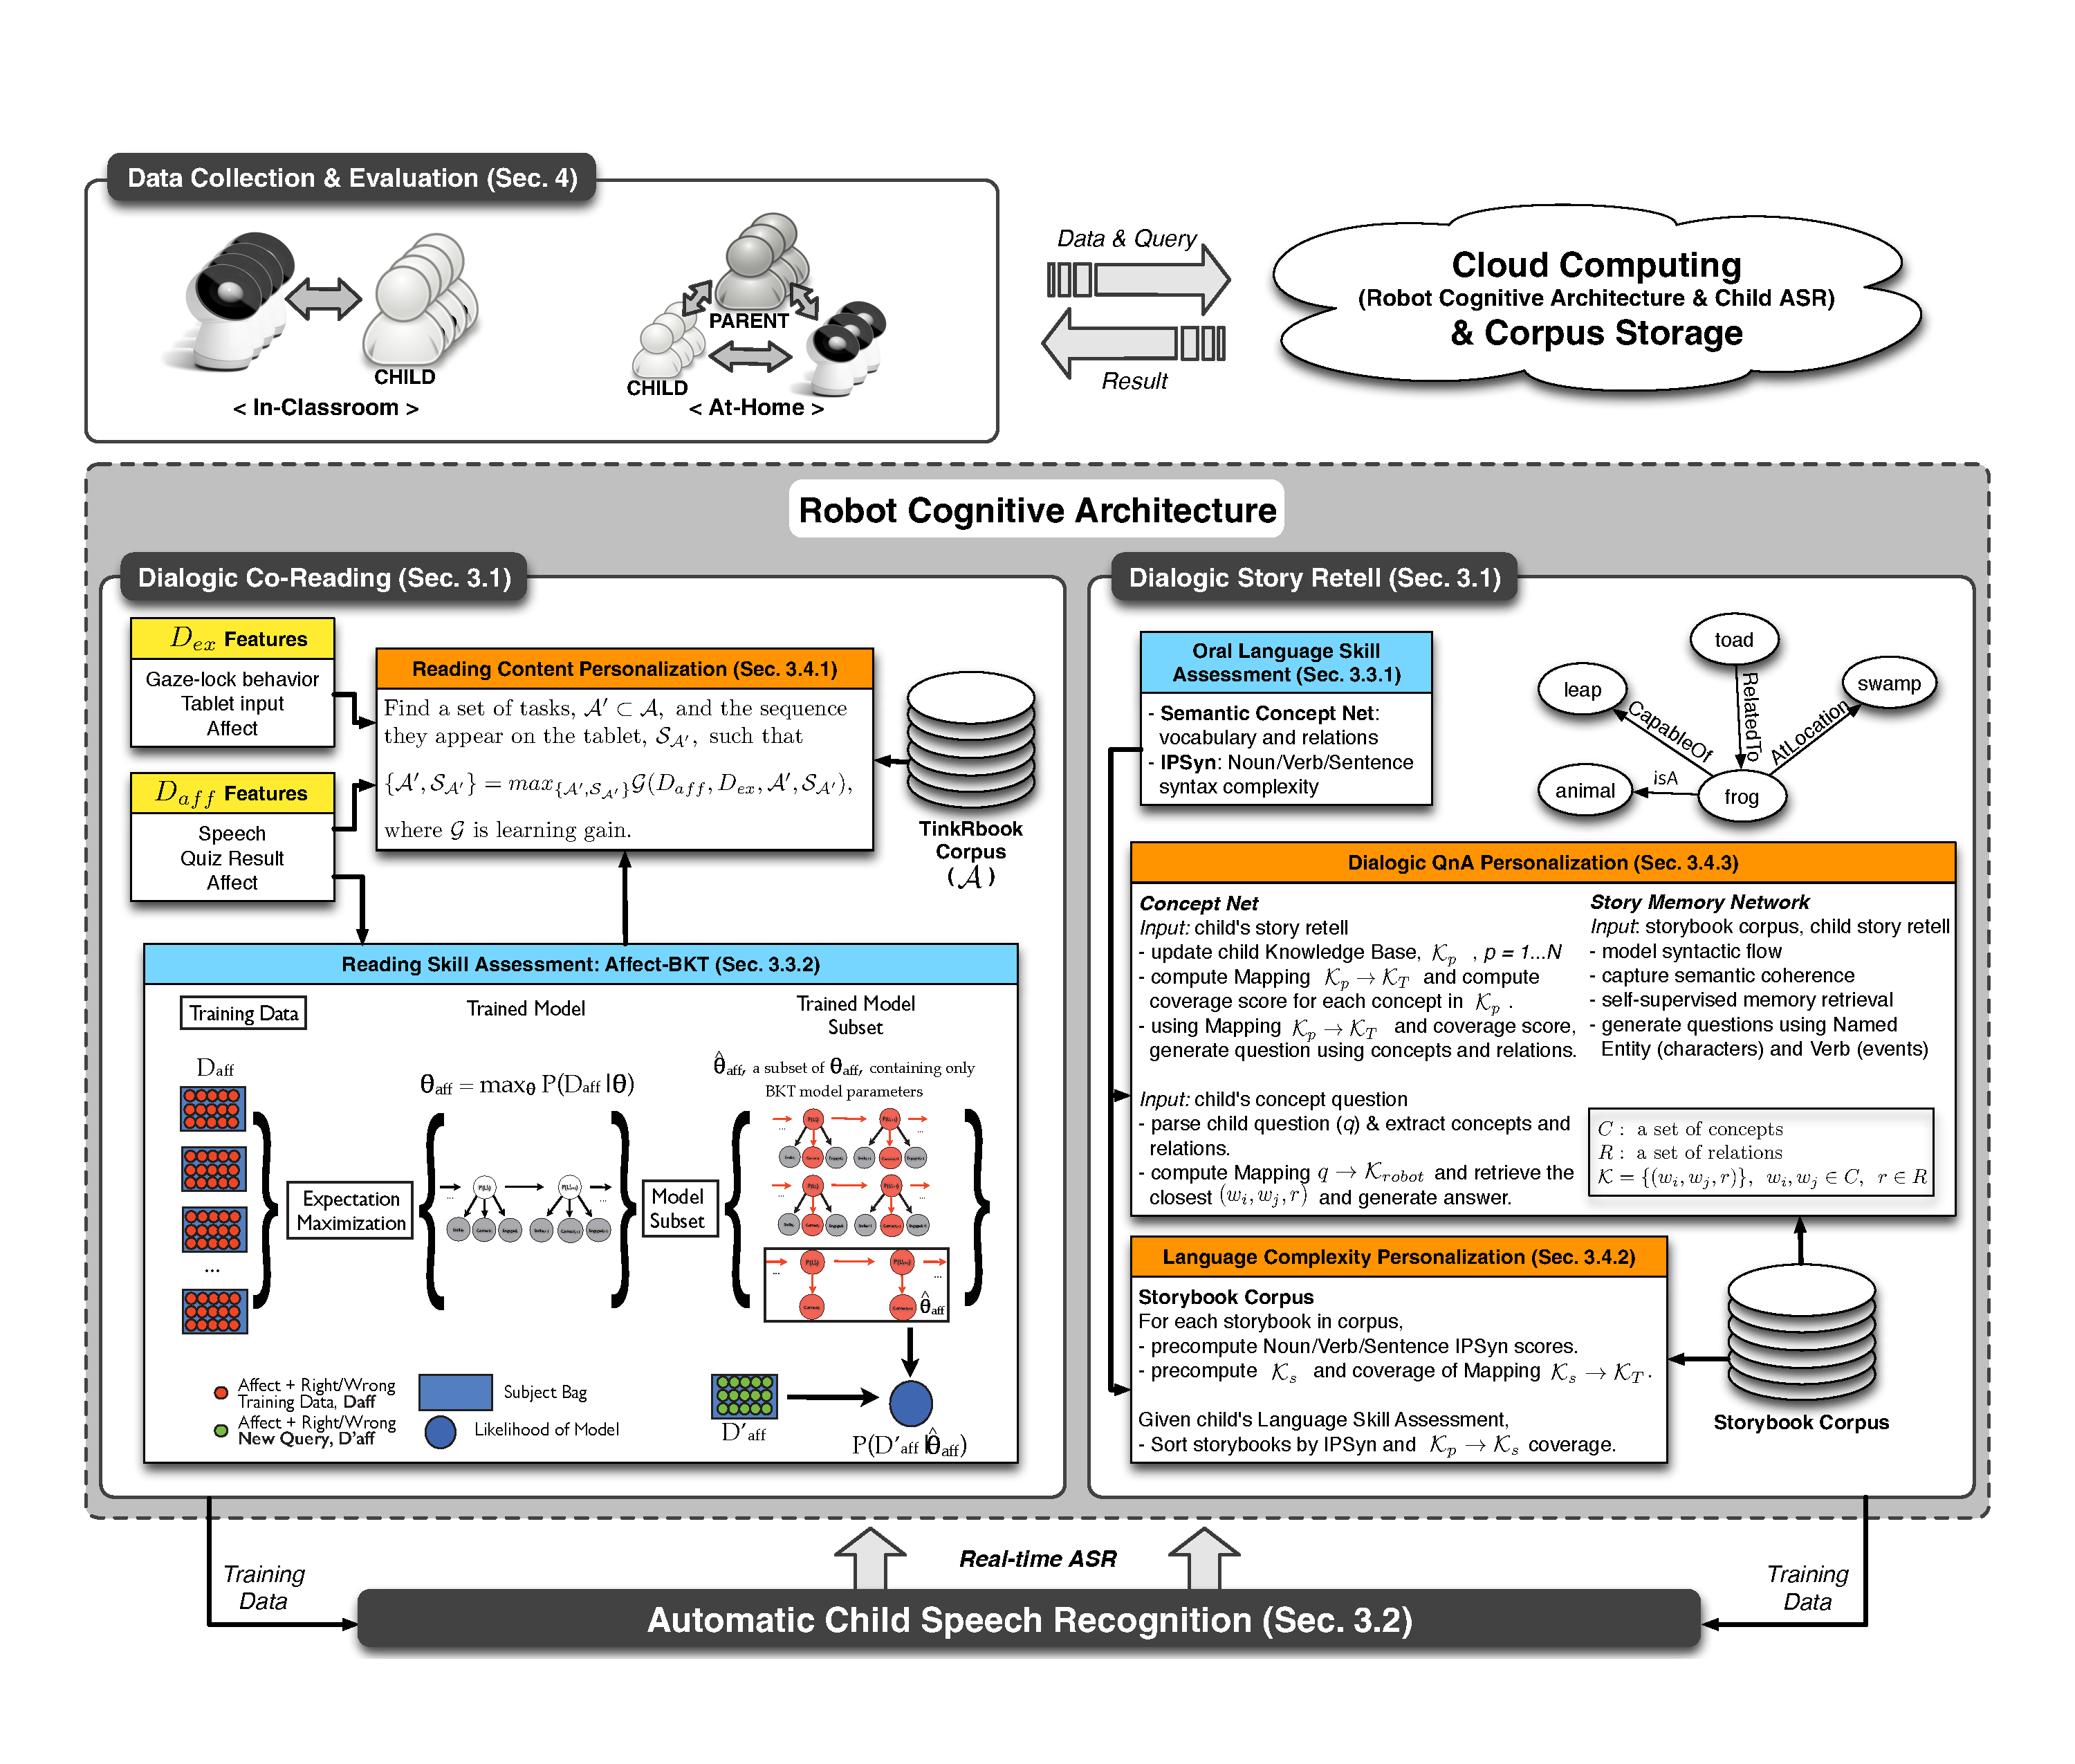
\includegraphics[width=\textwidth]{fig/NRI_arch.pdf}
  \caption{Personalized Learning Companion Robot system components: Innovative Robot Cognitive Architecture and Child ASR shall be developed and implemented as part of the cloud computing platform, which during the interaction our robot will send queries and receive real-time results (Section~\ref{section_proposedwork}). Our system shall enable online assessment of kindergarten-age children's reading and spoken language skills, provide personalized content and interaction solutions, and adapt the robot's language and dialogic behavior to the child. We will develop data corpus and evaluate our fully autonomous, collaborative, peer-like social robot system through multiple pilot and longitudinal studies in classrooms and at homes (Section~\ref{section_evaluation}).}
  \label{fig:system_arch}
\end{figure}

Building on our prior works (see Section~\ref{section_priorwork}), we will develop two categories of educational activity apps that integrate automatic speech recognition (see Section~\ref{section_ASR}) and automatic assessment of reading and linguistic skills (see Section~\ref{section_assessment}), with personalized content adaptation (see Section~\ref{section_personalization}). These apps will be used to both capture children's speech and video  to train our proposed computational speech and assessment models, and to capture data to assess children's language and literacy outcomes from the social robot intervention.

The interaction scenario involves having the social robot ``play" educational activates with a child like a peer with a tablet as digital interactive storybook. The two primary activities are outlined below, and there will be a library of content  of grade-appropriate children's stories associated with each, and leveraging assets developed from prior work to support multiple-month deployments (see Section~\ref{section_ipsyn}).  From these activities, the social robot system shall capture real-time audio, video, touch interactions, and app states on the tablet. This data shall be uploaded and stored in our team servers (see Data Management Plan), where the team can access it to train our novel computational models, to assess children's reading and language performance, and to adapt these activities and the robot's behavior to each child to optimize motivation, engagement, and learning. 

{\bf Personalized, Dialogic Co-Reading:} where children are invited to ``tinker" with, to touch, or to read text from single words to short sequences of words along with the robot who demonstrates, prompts, encourages, and asks questions to support dialogic reading (see Section~\ref{section_storyretell}).  The interactive storybook design builds upon our prior research in developing innovative interactive storybook apps, called TinkRbooks, to foster early literacy and language skills~\cite{Chang_Breazeal_2011}.  As the activity progresses, our Affect-BKT assessment algorithm models the children's reading skill (see Section~\ref{section_SAR}). Meanwhile, the system personalizes the digital stories and robot's questions to prompt and motivate the child, to reinforce comprehension, and to advance through a curriculum that balances challenge with mastery to optimize engagement.

{\bf Personalized, Dialogic Story Retell:} where a child first listens to a story on a tablet then retells that story to the robot. The child's retell of the story is transcribed using our ASR model (see Section~\ref{section_ASR}), and the transcript is automatically analyzed for linguistic skill and complexity using our automatic IPSyn tool (see Section~\ref{section_ipsyn}). Based on this linguistic assessment, the robot's dialogic questions (see Section~\ref{section_dialogicquestion}), story content, and linguistic complexity of that content is personalized to the child during the session and in subsequent sessions according to the principles of Vygotsky's zone of proximal development (ZPD;~\cite{Vygotsky_1978}) which requires tailoring language just above a child's current level of capability. The level is achievable with assistance from an expert (in this case the social robot) fostering learning and sustained engagement. The robot then tells a different story to each child, personalized accordingly.

These activities can easily be adapted to support either in-school scenarios where a robot and child play these activities together or a triadic interaction in homes where a parent-child-robot do these activities together. In prior work with the TinkRBook, for instance, we explicitly did in-home studies to study the design impact of TinkRability on fostering parent participation during story co-reading. We were able to show that this new design principle encouraged  parents to perform a range of positive emergent literacy behaviors (print referencing, dialog, and dialogic questioning) by 3 to 10 times more than with reading physical books~\cite{Chang_Breazeal_Faridi_Roberts_Davenport_Lieberman_Montfort_2012}. Additionally, children were observed to take a more active role in exploring the concept of text. With social robot triadic interactions, we observe that parents participate naturally as part of the group and similarly help to guide, highlight, motivate, and prompt their child~\cite{Freed_2012}. These design principles will be incorporated and further explored in the proposed work.

\subsection{Automatic speech recognition for young children}\label{section_ASR}

Innovative Automatic Speech Recognition (ASR) and Spoken Language Understanding (SLU) technologies will be developed to assess and diagnose children's comprehension of early literacy and language material based on storytelling, co-reading, and answers to the robot's questions.The goals are to: 1) develop innovative ASR algorithms for young children that are robust to age, gender, classroom noise and disfluencies, 2) create innovative SLU algorithms to extract useful information from children's stories and answers to story-related questions, and 3) develop and validate diagnostic assessments that probe vocabulary and syntactic structure acquisition related to conceptual understanding.

Since unconstrained recognition of children's speech can be prohibitively challenging~\cite{fainberg2016improving}, we will constrain the domain to assessment of comprehension of early literacy and language materials. We focus on co-reading out loud, story retell, as well as answering dialogic questions about the stories because: 1)  For our targeted age group, speaking is the main mode of communication as they are at the earliest stages of learning how to read and write. 2)  A corpus of annotated speech from children's reading, retelling, or responding to questions from a known library of books constitutes crucially important research data to advance testing and teaching approaches, as well as the development of theories of cognitive strategies. 3)  Oral language can not only determine accuracy, but also provide clues to help diagnose understanding of vocabulary, word usage, confidence, and focus.  

\begin{wrapfigure}{R}{0.35\textwidth}
  \centering
  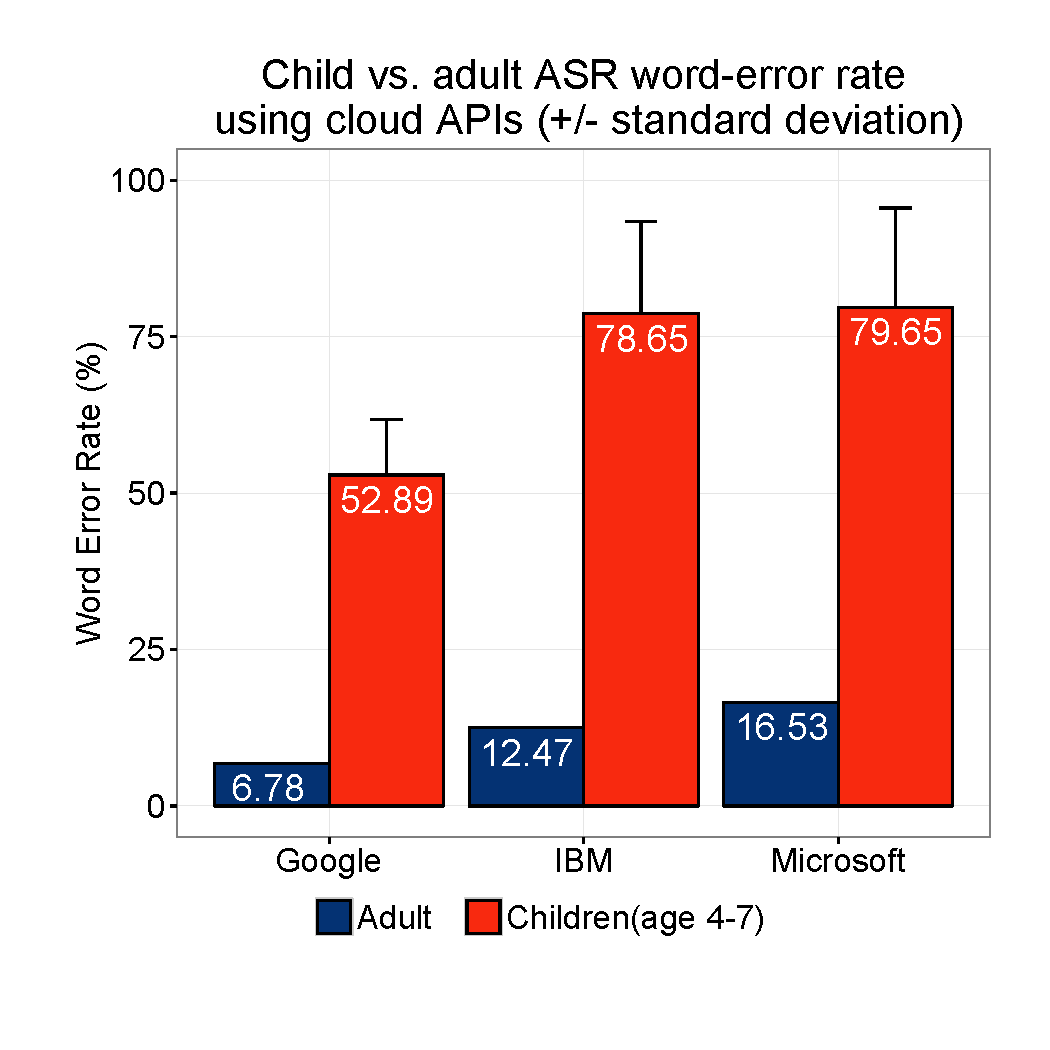
\includegraphics[width=0.35\textwidth]{fig/asr.pdf}  
  \caption{The performance of the state-of-the-art ASR tools is far from functional on child speech.}
  \label{fig:asr}
\end{wrapfigure}

Achieving the proposed goals presents several important challenges, including speech and language variability as a function of age, sex, socio-cultural factors, cognitive load, skills, and individual differences. Automated methods need to adapt robustly in the presence of such variability, while using information in the variability to discriminate among various learner states. Compared to adult speech, child speech is more challenging~\cite{price2009assessment,fainberg2016improving} due to (a) more omissions, substitutions, and mispronunciations, (b) shorter words that make discrimination more difficult, (c) more creative word use, (d) diversity in anatomy and physiology and developing motor skills, (e) larger variation in spectral and temporal parameters, and (f) larger number of disfluencies.  

The MIT team organized a workshop\footnote{IEEE RO-MAN 2016 Workshop on Enabling Long-Term Child-Robot Interaction: \url{http://web.media.mit.edu/~haewon/Roman-LTCRI/}} in 2016 to discuss the important enabling technologies for long-term child-robot interaction. The researchers elected child speech recognition as the top-most limiting factor in advancing child-robot research. The current state-of-the-art ASR models are mainly trained and evaluated on adult-speech corpora, such as the LDC\footnote{Linguistic Data Consortium: \url{https://catalog.ldc.upenn.edu/byproject}} training dataset. While various tools report achieving close to a single digit word-error rate (WER) on adult speech~\cite{saon2015ibm,xiong2016microsoft}, there is still no technology for child speech with accuracy rate above 50\%. Figure~\ref{fig:asr} shows our analysis of the performance of several cloud-based ASR APIs on child speech. We tested with a corpus of 5.5 hours of storytelling speech samples from 75 preschool and kindergarten children (ages 4--7 (5.13$\pm$0.64)), collected throughout our previous NSF projects. WER of an adult narrating a story used in prior studies is presented as a baseline for comparison. Overall, child-speech recognition rate was significantly lower than adult speech for all APIs (p < 0.0001), and their performance is unacceptable from a practical standpoint. An in-depth analyses of child speech ASR was recently published by Kennedy et al.~\cite{kennedy2017child}.

% \newcolumntype{S}{>{\centering\arraybackslash}m{1.5cm}}
% \newcolumntype{M}{>{\centering\arraybackslash}m{1.5cm}}
% \newcolumntype{L}{>{\centering\arraybackslash}m{1.8cm}}
% \begin{table}[h]
% \scriptsize
% \captionsetup{font=scriptsize}
% \resizebox{1.4\textwidth}{!}
% {\begin{minipage}{\textwidth}
% \begin{tabular}{S|S|S|S|S|S}
% Dataset (grade level) & \# of participants (female ratio) & Age (mean$\pm$sd) & Total \# of storytell sessions & Total sample length (hr:min:sec) & NSF grant\\
% \hline
% Dataset1 (Pre-K,K1) & 17 (0.59) & 4.88$\pm$0.49 & 177& 2:03:07&NSF CCF-1138986\\
% Dataset2 (K1,K2) & 40 (0.55) & 5.20±0.76 & 69 & 2:03:30 & NSF CCF-1138986\\
% Dataset3 (K2) & 18 (0.39) & 5.22±0.44 & 66& 1:25:22& NSF IIS-1523118 \\
% \hline
% Total & 75 (0.52) & 5.13±0.64 & 312 & 5:31:59 &\\
% \end{tabular}
% \caption[Table caption text]{Speech samples collected through storytelling activities at  different preschools and kindergartens.}
% \label{table:name}
% \end{minipage} }
% \end{table}


Most previous work on children's speech has focused on exemplar productions. We propose to focus on speech variants under co-reading and storytelling learning/assessment conditions. Understanding developmental changes in children's speech has helped us devise strategies for dealing with acoustic mismatch between different age groups and for designing robust ASR for assessment~\cite{alwan2007system}. We will investigate how speech and language cues emerge as learning develops by quantifying variation in segmental and suprasegmental properties (F0, duration) in a variety of learning and assessment scenarios. Understanding unconstrained spoken language is far from solved, but we envision progress towards this goal through 1) constraining and structuring the target application domain, and 2) using good prior models combining cue-based machine learning methods (exploiting lexical, prosodic and discourse information), and rule-based methods (within a pedagogically sound assessment framework).

In contrast to traditional unsupervised or fully-supervised adaptation, we will draw on datasets as needed for particular purposes. This will be particularly important for modeling the proposed populations, since children's use of language changes as they learn to tell more elaborate stories. We believe that the proposed techniques will generalize to other domains and result in novel speech modeling paradigms that go beyond the conventional ASR problem of phonetic transcription. Below we describe the tasks proposed including: Infrastructure (collecting additional data, adapting existing data structures and interfaces), Speech Processing (robustness to speaker and pronunciation variability, to noise, and to disfluencies), Modeling storytelling (assessing use of language, and student modeling), and Evaluation.

{\bf Infrastructure.} In addition to the acoustic model training, we will need data on what words children use in retelling stories and how they use them in order to train language models that will constrain the lexical search during recognition. For both the acoustic and language modeling uses, the data will be transcribed at the word level and annotated with the metadata (e.g., fluency ratings, correct/incorrect and other item ratings). (See Section~\ref{section_ipsyn} for our prior work in automatic crowdsourced transcription of children's stories).

{\bf Speech Processing.} Larger intra- and inter-speaker acoustic variability for children, relative to adults, requires that acoustic models account for larger acoustic parameter ranges and temporal and spectral variability. Dealing with environmental noises in the classroom is also essential for robust ASR. Disfluency associated with children's speech is another confounding factor as it creates complexity in acoustic modeling as well as in speech decoding using recognition grammars or language models. In order to address these major challenges, we will develop novel and robust conversational interfaces. To accommodate various assessments, we need to improve ASR accuracy and add new measures such as reaction times. Since our technology development relies critically on scaling up systems for a variety of children under several conditions, we suggest a phased iterative design approach. We will rely on mock-up design experimentation for the proposed assessment framework, especially in the initial stages, with transitioning interface design and automated analyses.

    
{\bf Robustness to Acoustic Variability.} Inter-speaker variations of acoustic characteristics of speech sounds constitute a major cause of performance degradation in ASR systems. Such variations are caused by differences in the vocal apparatus and speech motor control. To maintain ASR robustness against speaker variability and developmental changes, speaker adaptation and normalization techniques are applied to reduce spectral mismatch between training and testing utterances~\cite{leggetter1995maximum}. We propose to use subglottal-based normalization for rapid speaker adaptation~\cite{arsikere2014frequency}. In addition, we will apply constraints imposed by speech production theory to model speaker variability. The proposed techniques are transformative in that they will require short amounts of data (a few seconds) to perform adaptation utilizing articulatory constraints. 

{\bf Robustness to Background Acoustic Noise.} In addition to challenges related to the variability of children's speech, classrooms can be unfavorable environments for ASR because of the high degree and non-stationarity of background noise. Noise, for example, could arise from other speech-like signals (e.g., the cocktail-party effect) or from non-speech-like signals (e.g., air-conditioning noise). We will develop noise-robust ASR systems based on three approaches: noise-robust feature extraction, variable frame rate analysis, and missing feature theory.
    
The goal of ASR feature extraction is to design front-end features which retain discriminative information while suppressing information which may introduce confusability into the recognizer. In~\cite{strope1997model,strope1998robust} we offer successful front-end features, motivated by the human auditory system, which isolate and enhance spectral peaks. Another approach to noise-robust ASR, also motivated by human speech perception, is variable frame rate (VFR) analysis~\cite{zhu2003non,you2004entropy}. In VFR, features are sampled adaptively according to the discriminative importance of speech segments. In the proposed work, we will derive a channel-specific VFR framework, which will adaptively sample feature components differently based on the information present in various frequency channels. In addition, we developed noise-robust ASR utilizing missing feature (MF) theory. In MF-based systems, unreliable spectral components are located via mask estimation, and compensated for accordingly. There exist two types of MF approaches: data imputation and marginalization. Data imputation reconstructs unreliable spectrographic (time/frequency) data prior to recognition~\cite{borgstrom2009missing} whereas marginalization deemphasizes the effect of unreliable components during  recognition~\cite{cooke1997missing}. A major and challenging component of MF-based systems, however, is mask estimation~\cite{tan2014feature}. We will develop these noise-robust techniques and apply novel statistical model-based methods to derive improved reliability masks.

 	{\bf Robustness to Disfluency.} Disfluencies such as filled pauses, repetitions, false starts, hesitations and repairs are inherent in spontaneous speech interactions. Although disfluency detection is relatively easy when one has prior knowledge of the correct utterance (e.g., read speech), it has not yet been well addressed in spontaneous speech recognition. In the proposed work, we need to deal with spontaneous speech by dividing the problem of disfluency processing into two sub-problems: (1) disfluency detection in the input utterance and (2) disfluency assessment by post processing of the recognized utterance. The disfluency detection problem will initially deal with the creation of a recognition dictionary that includes lexical entries of disfluent sound objects such as partial words and non-speech sounds (e.g., lip-smacking, laughing, etc). Depending on how they were produced, these sound objects will be phonemically transcribed or entered as individual lexical objects using pre-defined transcription symbols. The transcribed data will be utilized for acoustic model training of disfluent sound objects.
    
{\bf Robustness to Pronunciation Variability.} In addition to acoustic modeling to reduce the effects of speaker variability, improved pronunciation modeling is also required due to large lexical pronunciation variability in young children (e.g.,~\cite{tepperman2006pronunciation}). Pronunciation variants of target words will be added to the recognition dictionary based on observed frequency in the training data. Such a multiple pronunciation dictionary can be augmented by applying hybrid pronunciation representations using variable length units (e.g., context-dependent phones, syllables, words) for better ASR performance. Once an optimal lexicon file has been derived for the domain, the multiple pronunciation dictionary can be used to realign the training speech data and train improved acoustic models. As more data are accumulated we will derive a rule-based system for generating possible pronunciation variants, based on age, in order to absorb some potentially unseen pronunciation variants and to enhance the multiple pronunciation dictionary.

Transformative results are expected from: a) pronunciation modeling and speaker adaptation techniques appropriate for children of various competency levels in English, b) child-specific language modeling including syntax, non- lexical events, and discourse phenomena as well as limited-domain natural-language processing for assessing comprehension, and c) novel noise-robust ASR algorithms.


\subsection{Automatic Assessment Algorithms}\label{section_assessment}

In our prior work, assessment of children's oral and reading skills were conducted offline, after children interact with a robot, which significantly hindered real-time robot behavior and curriculum personalization. This proposed work will enable online adaptation of these algorithms through innovative child ASR, collection of diverse corpus to train and improve affect knowledge models, and incorporating active learning methods to achieve real-time assessment and personalization.

\subsubsection{Oral Language Assessment}\label{section_languageassessment}
We shall build upon our prior work in developing IPSyn-based computational methods (Section~\ref{section_ipsyn}) for assessing children's oral language development while the interaction is happening. The robot will generate just-in-time dialogic questions based on this automatic assessment. For this proposed work, we shall also extend this system to investigate automatic ASR transcription using the story retell as a context to constrain the ASR models. We shall compare the performance of this automatic system to existing human crowdsourced transcriptions. 

\subsubsection{Reading Assessment}\label{section_readingassessment}

% \begin{wrapfigure}{r}{0.42\textwidth}
%   \centering
%   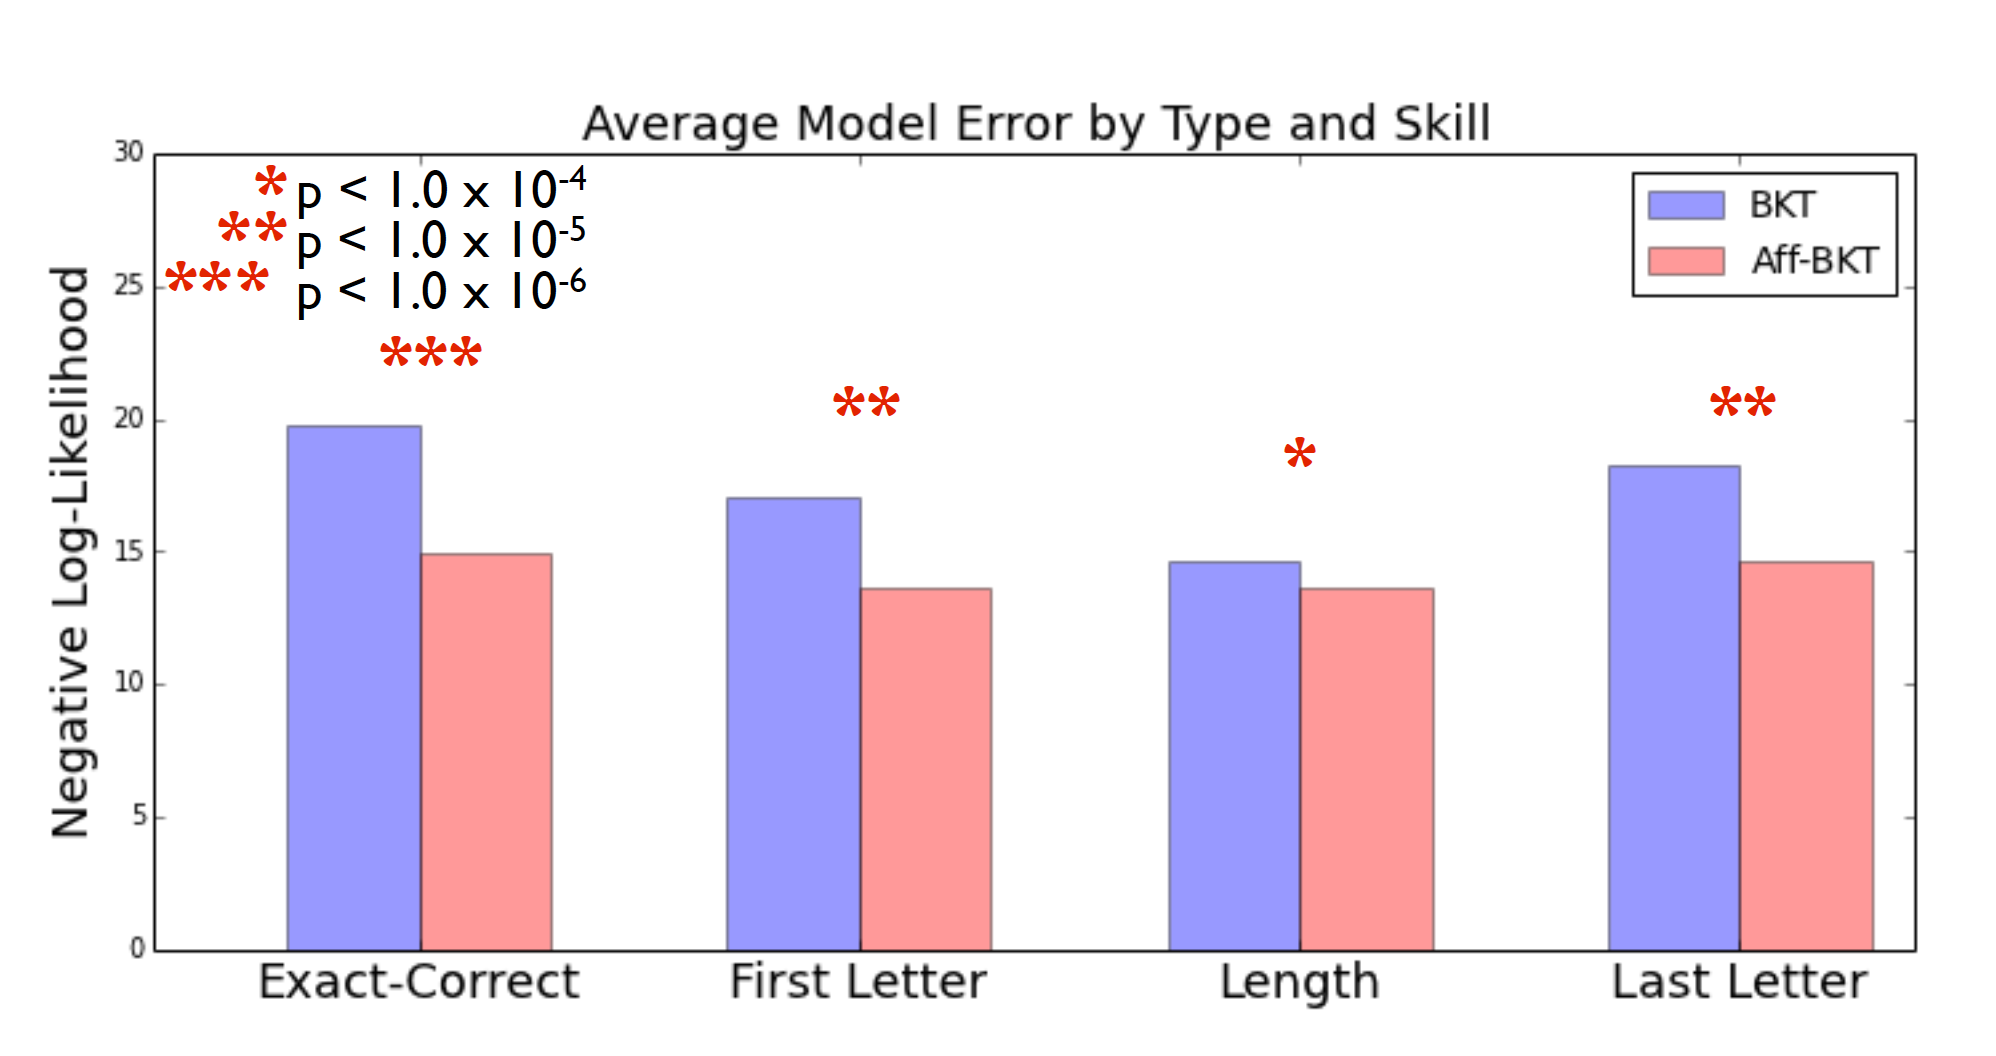
\includegraphics[width=0.4\textwidth]{fig/affect-bkt.png}  
%   \caption{Mean error estimates of BKT and Affect-BKT models by skill. Affect-BKT significantly decreases model error compared to traditional BKT.}
%   \label{fig:affectBKT}
% \end{wrapfigure}

Recall in our prior work (Section~\ref{section_SAR}), we showed that using affective information to create Affect-BKT model outperformed traditional BKT in assessing single-word reading skills~\cite{Spaulding_Gordon_Breazeal_2016}. 
%We focused on a single word reading task, modeling a set literacy skills known as ``alphabetic principle" skills~\cite{Byrne_Fielding-Barnsley_1989, Liberman_1989} to train four models, each corresponding to a word-reading skill (denoted as Exact-Correct, First-Letter, Length, and Last-Letter in Figure~\ref{fig:vocabulary}-(c)). 
Given our promising results with our Affect-BKT reading assessment algorithm  for young children, we propose the following extensions to develop a more advanced model that shall:

{\bf Span to Multi-word reading tasks.} Our previous work developed Affect-BKT models that more accurately assessed student's performance on foundational, one-word reading skills. We propose to extend these results to more advanced reading skills, e.g., assessing phrases and complete sentences.

{\bf Expand beyond tactile based inputs} {\bf to spoken inputs.} Our previous work relied on a child identifying (by tapping on a touchscreen) the written form of a spoken word to assess reading. More appropriately, though, reading is assessed by having the child speak a given word from its written form. The development of a robust child ASR model (Section~\ref{section_ASR}) will enable us to incorporate this more appropriate model of reading assessment into our methods.

{\bf Employ active-learning approaches} to improve algorithm convergence rate and accelerate model improvement. Generally speaking, Affect-BKT models improve with additional data. But collecting additional data often requires asking additional questions or prompting the child for new demonstrations of a skill. Maintaining child interest over a 20--30 minute educational interaction with an autonomous robot remains a challenge, which often limits the amount of useful data that can be collected in any single session. By employing an active-learning approach, we will ensure that the data we do collect provides the maximum expected inferential power, allowing the Affect-BKT models to accurately estimate a child's skill under real-world conditions and with practical data constraints.

{\bf Incorporate hierarchical and interdependent data structures} for skill inference. Previously, our models assumed that the alphabetic principle skills were mastered independently. Affect-BKT models are trained from the right/wrong quiz results and the affective QnA-interval data ($D_{aff}$) via expectation maximization, resulting in a set of learned model parameters, ${\theta}_{aff}=max_\theta P(D_{aff}|\theta)$ (see Figure~\ref{fig:system_arch}). We shall extend the Hidden Markov Model (HMM) structure of our previous Affect-BKT models to a Hierarchical Hidden Markov Model (HHMM) that captures the relationships and dependencies between skills and higher-order concepts essential to literacy development. 


{\bf Personalize to individual students.}  Our previous work developed Affect-BKT models trained on data from 38 children. By incorporating more diverse sources of real-time, real-world data as well as deploying the active-learning algorithms discussed above, we shall extend our work to develop personalized assessment algorithms, trained on a specific child's unique patterns of affective expression, attention, and prior knowledge.

%TODO extract core information from the following.
%Our proposed child assessment algorithms shall receive input from several multi-modal data sources to estimate children's reading and literacy skills. This includes: gameplay records via tracked touch screen inputs, speech sample audio data used for training the ASR model as well as for assessment and as input for the story game activities, facial recognition data to identify individual child participants to enable social bonding and long-term personalization, facial orientation and gaze direction data to assess, e.g., whether a participant is ``on-task", their level of engagement, and which aspects of the task capture their attention, and facial expression recognition data to identify child affect using the Affdex SDK, a commercial, FACS-based affect-analysis tool trained on data from over 2.7 million faces in 75 countries~\cite{swinton2012measuring,mcduff2012affectaura}. These data serve as inputs to our inference algorithms, enabling fine-grained, continuous student assessment of reading and associated literacy and linguistic skills. The outputs shall drive personalized adaptation of our custom apps and the mentoring interface to keep students in a state of Flow in which they are highly engaged in a task at an optimal challenge level~\cite{Csikszentmihalyi_1997}. 


\subsection{Personalization Algorithms}\label{section_personalization}

We shall iteratively develop a set of personalization algorithms based on human factors research and building on our prior work. Personalization algorithms shall incorporate both student performance data via assessments, as well as interpersonal cues such as affective data for valence, attention, and engagement, facial ID, and SLU analysis of prior recorded audio.

\subsubsection{Reading Content Personalization}\label{section_contentpersonalization.}
Based on a scope and sequence of target words and short word sequences per curriculum, our co-reading TinkRbook apps shall automatically adapt the challenge level of stimuli presented to the child. A child’s current skill, assessed by Affect-BKT using the child’s demonstrated skills (speech and app interaction) and affective states (a strong indication of confidence and engagement level), will be compared to the stimuli that are part of the curriculum scope and sequence. As part of our iterative human factors research in the first 3 years of the project, we shall develop an optimization algorithm for real-time adaptation of stimuli levels to maximize the child’s learning gain. Namely, inferring the combination of tasks with varying difficulty to effectively encourage and challenge each child, and deducing the sequence and location of how those tasks (individual apps) appear to children on a tablet. The difficulty of each task shall be expressed as a probability of learnability with the child’s current skill level, learning speed, and engagement as inputs to the function. Each child’s exploratory behavior will be used to develop an inference model to predict which app the child will select next, which will determine the tablet app placement strategy given a set of optimized tasks (see Figure~\ref{fig:system_arch}).   

\subsubsection{Oral Language Complexity Personalization}\label{section_storypersonalization}
The complexity of the stories during the story-retell task will be personalized to the currently assessed language skill of each child (i.e., their ZPD). Based on a scope and sequence within our specified story corpus (informed by co-PI Bailey and consultant Gottwald), we shall compute the linguistic complexity levels of each story according to their noun, verb, sentence complexity using the IPSyn score as a standard measure. Children's utterances will be similarly scored and assessed using the IPSyn tool by sentence type (fragments, questions, imperatives, complex, etc.).  Secondly, item-based patterns will be traced for their frequency. This process takes into account the growth of children's vocabulary knowledge and the relationships between their exposure to specific constructions and the occurrences of constructions in their own speech. We shall also compute a distance metric as a measure of the child's current demonstrated linguistic skill level relative to that of the stories in the corpus. The selection of a story for a given child is based on the (i) complexity level of synonymous adjectives, verbs, and nouns of each character and scene; (ii) complexity of the generated sentences to include specific syntactic constructions. While several automatic story-generation algorithms have been proposed in the past -- e.g., the Novel Writer system that generates murder stories within the context of a weekend party~\cite{klein1973automatic} to ground-up approaches leveraging non-deterministic simulations~\cite{leon2014creativity}, they have not addressed children stories, nor personalized content complexity. As part of our human factors research, we shall experiment with personalized story selection based on this distance metric, using engagement via facial expression as well as change in quality of children's story retell over time. 
 
\subsubsection{Personalized Dialogic QnA Generation}\label{section_dialogicquestion}
In prior work (Section~\ref{section_storyretell}), we were able to show the benefits of having a robot ask dialogic questions during a storytelling task. For example, %Figure~\ref{fig:dialogic} shows that 
children who responded to the robot's dialogic questions were more likely to use target vocabulary words and phrases in their story retell, and they tended to tell longer stories even after two months. These results suggest that the presence of dialogic questions helps children engage in the activity and focus their attention on specific elements of the story. 

% \begin{wrapfigure}{r}{0.45\textwidth}
%   \centering
%   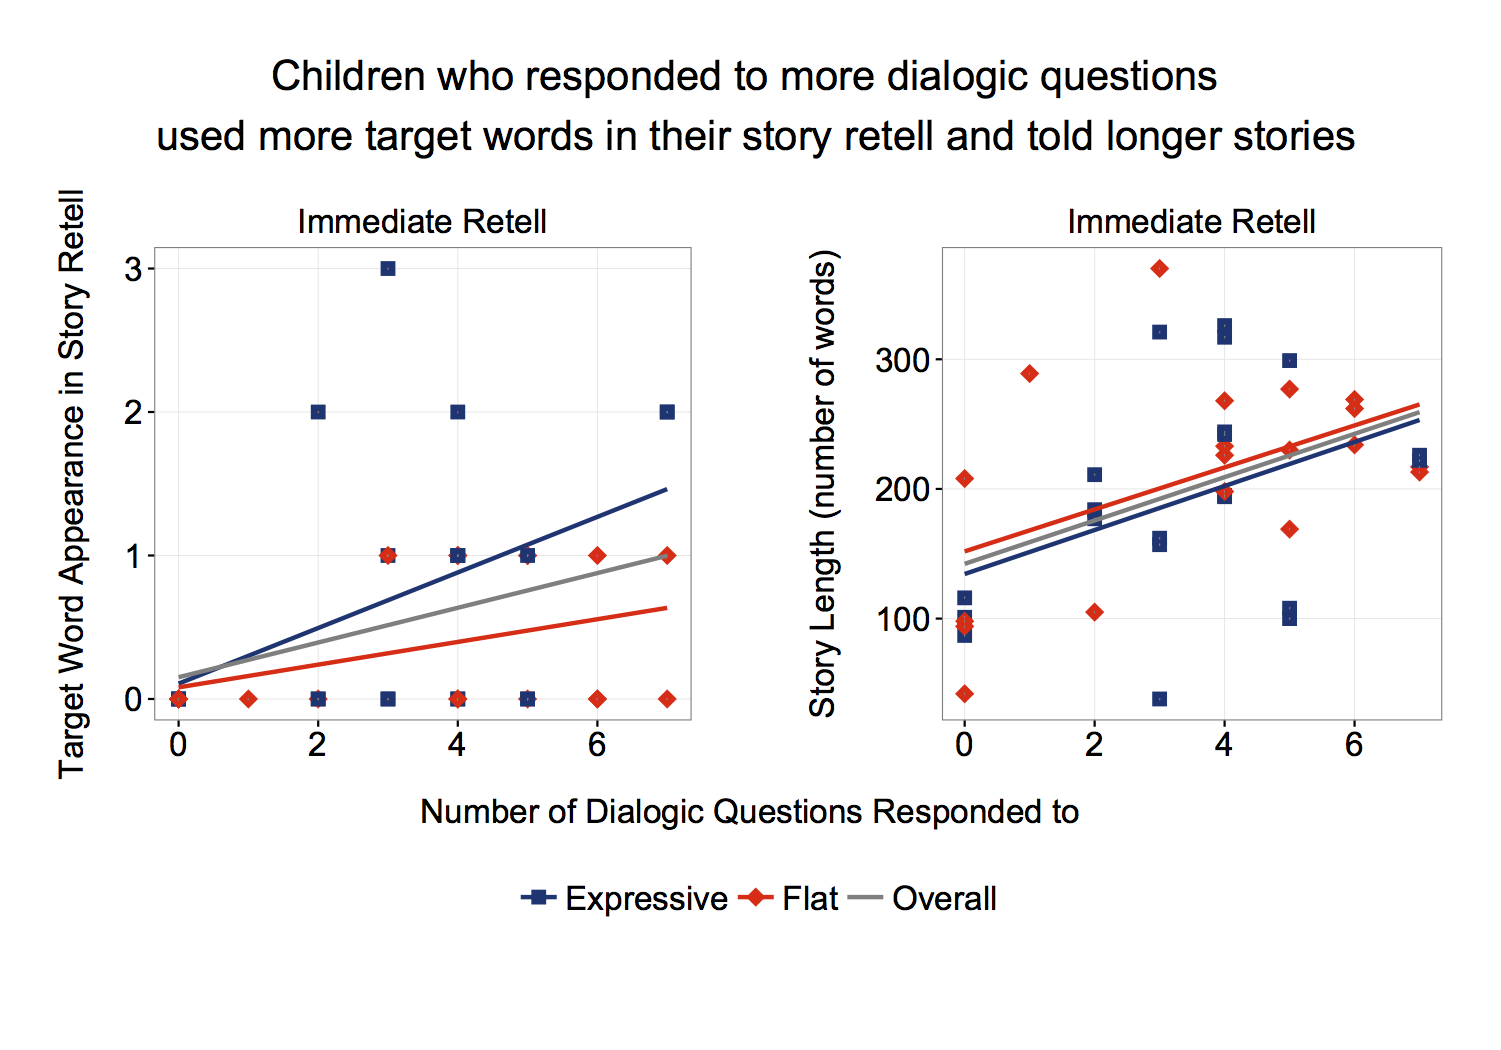
\includegraphics[width=0.43\textwidth]{fig/cyber4_dialogic_length.png}  
%   \caption{Dialogic questions asked by the robot during storytelling effectively engages children in the activity and focuses their attention to specific learning elements.}
%   \label{fig:dialogic}
% \end{wrapfigure}

While previous work used a pre-defined set of questions for all children, we shall develop automatic question generation algorithms for probing children's concept understanding and perspective taking. Dialogic questions will be generated in real-time and asked during and after a child's and robot's storytelling (see Figure~\ref{fig:system_arch}). More specifically, we focus on developing the following:

\textbf{Concept Net:} Given a set of concepts $C$ and a set of interlingual relations $R$~\cite{speer2012representing}, a knowledge base (KB) is a collection of a set of two concepts (words or noun phrases) and their relation, i.e., $\mathcal{K}=\{(w_i,w_j,r)\}$, $w_i,w_j\in C$ and $r \in R$. Informed by the curriculum, a target KB, $\mathcal{K}_T$, is given as a guide. When the robot hears a child telling a story, it starts updating the child's KB, $\mathcal{K}_p$, a robot's belief of the child's semantic network. The idea is to compare  $\mathcal{K}_p$ to $\mathcal{K}_T$ and find concepts that exist in both but missing specific relations that exist in $\mathcal{K}_T$ but not in $\mathcal{K}_p$, to generate a set of productive concept-relation questions. For instance, if a child tells a story of a boy who goes in an adventure to find his missing pet frog, the robot may probe for ``{\it frog}--LocatedNear--{\it swamp}" and generate a question, ``where do you find frogs?". 
 
% and a likelihood of those relations ($\mathbf{l}$). A robot's belief of a specific user's semantic network, $\mathcal{K}_p$, starts from a blank slate and is developed while listening to the child's storytelling over a long-term. Each $\mathcal{K}_p$ is associated to a child through a face-recognition algorithm. Given a new speech sample $s$, a likelihood of two words $w_i,w_j\in s$ having a relation $r_k$ is updated, $\mathcal{L}_{ijk}(w_i,w_j;r_k|s)$, through relation extraction and relaxation~\cite{havasi2007conceptnet}. In order to resolve {\it weak} concepts in $\mathcal{K}_p$ that exist in $\mathcal{K}_T$, the robot will generate word-relationship questions to actively probe a child's comprehension of the concept (example: from ``{\it frog}--LocatedNear--{\it swamp}", a question ``where do you find frogs?" can be generated). The scope of each child's semantic network will be evaluated by using it towards answering a set of vocabulary questions within the curriculum. All children's $\mathcal{K}_p$ combined, we shall gain insights into kindergarten children's general concept level after the completion of the studies.

%Using context-based inference model to train and update an individual child's concept network, we shall depict the relations between the terms that appear in a child's story. We will adapt interlingual relation representation method in~\cite{speer2012representing}, such as those depicted in Figure X. When a targeted concept knowledge is absent, the robot will generate word relationship dialogic questions using this relational knowledge representation to actively probe a child's comprehension of a concept. (example: ``where do frogs live?") 

% \textbf{Generate leveled up syntax structure:} After an initial phase of syntax level assessment using the IPSyn analyzer, the robot will generate 

% a next-level syntax structure by reusing a child's own sentences. (example: child - ``Boy is sleeping. Frog is jumping out."  -> robot -``Okay, the boy is sleeping and the frog is jumping out. And then?")

\textbf{Story Memory Network:} Our robot storyteller shall automatically generate story-context questions for the stories in our corpus. First, we will track story's characters/scenes (named entities) and events (verbs) through explicit memory representation. Using memory network, we shall model syntactic flow of the story, detect semantic coherence, and develop word-level and sentence-level memory representation using {\it window memories}~\cite{hill2015goldilocks}. In addition to asking questions during its storytelling, the robot will, as part of its backchannel (listener response) feedback, prompt children with questions while they are telling a story. These questions will be more open-ended since tracking a story plot and asking questions at the right timing is difficult in real-world interaction (the rule-of-thumb is, any listener feedback should happen within 500ms of detecting backchannel opportunity~\cite{park2017hri-bc}). Hence, we will use shorter {\it window memories} and generate questions probing for character's internal landscape and change of perspectives (example: ``How did the boy feel when the frog was gone?"). The objective is to prompt and encourage children to think about the perspectives of the characters and the events that occur around them and incorporating them into a story narrative. 

Through longitudinal studies, we shall study whether children answering dialogic concept/story questions has long-term effect in language learning as well as engagement. For evaluating a child's concept growth, we will define a coverage score from the mapping $Map: \mathcal{K}_p \rightarrow \mathcal{K}_T$. Furthermore, all participants' $\mathcal{K}_p$ combined, we shall gain some insights into kindergarten children's general semantic network growth.

%Children will be evaluated whether they correctly answer story questions and whether incorporate sentences that reflect internal landscape of the characters or themselves in their future stories.



%https://research.fb.com/projects/babi/

%The same concept-probe model will be used to assess the quality of questions generated by children, as questions generated by a learner is often a strong indicator of the level of comprehension (citation). %TODO
% * <cynthiab@media.mit.edu> 2017-01-25T13:09:23.939Z:
% 
% > citation)
% missing citation
% 
% ^.

\section{Evaluation}\label{section_evaluation}

In order to address our 4 primary research questions outlined above, we will develop the proposed technologies, integrate them with a commercial social robot platform to support the required scale of deployments, and conduct a series of multi-site studies with the following protocols, ranging from short, iterative pilots, to a 3-month deployment in homes with Kindergarten age children (Year 3), to in-classroom deployments lasting for 4 months in Kindergarten classrooms (Year 4).  See Human Subjects Plan.

\subsection{Robot Testbed}\label{section_robot}

We shall use a commercial social robot with SDK to support the proposed research and studies. (see Facilities, Equipment, and Other Resources). As in prior work, we shall integrate a tablet as an interactive digital storybook. The number of robots, length of deployments, and required reliability mandates the use of a commercialized system over laboratory prototypes. Fortunately, commercial social robots are entering the consumer market. We intend to use the Jibo robot (www.jibo.com) given its technical capabilities support the requirements of this proposed work. The robot is very affordable, roughly the price of a high-end tablet computer, and the Lead-PI will have 20 units delivered to her lab. Presently, it is the only social robot with sensing, expressive, and SDK capabilities that meets our project requirements. Namely, it is safe to interact with no pinch points, it is of high appeal to children, it is highly expressive with several degrees of freedom, it is wifi connected to a cloud backend, has stereo cameras, a microphone array for sound localization, dual speakers, a color touch screen, touch sensors on its head, can run on battery power (up to 1 hour) or be tethered for power. The SDK supports a suite of capabilities in order to author new ``skills" for the robot including specifying behavior logic, authoring of new body movements or screen animations, as well as producing text-to-speech with tools that support sculpting prosody. The robot is capable of face detection, face recognition, and speaker identification within a limited number of people. It also supports facial expression recognition. (See Letter of Collaboration.) See Data Management Plan for a description of the cloud-connected backend and database that we shall use for data collection, storage and sharing.


\subsection{Pilot Deployments for Data Collection and Iterative Development}

In years 1-3 we will do a series of short  length pilot deployments with the primary purpose of gathering data to train and continually iterate on our proposed technologies and systems.  The long-term deployment of the robot will push the envelope of autonomous interactions with social robots in an educational settings. We anticipate mechanical, software and network issues that will arise in these challenging environments. A dedicated person will accompany these early pilots and deployments to discover such issues on-site. Any issues that need to be dealt with in the lab will be promptly addressed as well. Furthermore, as we move to longer deployments during this phase, we will closely monitor the engagement levels of the children during extended interaction, via close collaboration with the teachers, in person inspection and video recording analysis. This will enable the full analysis of the engagement, entertainment and social aspects the interaction with the robot will have.

{\bf Protocol.} These pilot deployments are informal and short in duration. They are intended to bring the social robots into the target environments (Kindergarten classrooms and homes) primarily to engage children in the playful activities that are under iterative design and development with the robot. A key objective is to receive feedback on these activities, the behaviors and interaction design of the robot, and importantly, to  collect the necessary data to train our various models. 

{\bf Data Collection and Analysis.} As detailed above, during the development phase of each of the individual components (i.e., automatic reading and language assessment tools, automatic question-generation algorithm, ASR and SLU models, and activities with the autonomous social robot learning companion), we will collect the associated aforementioned data, analyze it with practical and performance measures, and refine and iterate each component. More specifically, the textual transcription of children's stories will be documented and analyzed at each stage of the ASR model iteration, so as to inform others who wish to extend and improve the model. The story analysis tool shall be iterated upon to focus on initial assessment of language skills (i.e., vocabulary and grammatical structure). We believe that more complex cognitive and social concepts can be extracted and analyzed via children's storytelling as well using SLU. Our efforts shall provide structured textual datasets to support this  research. The story-leveling algorithm will also be iteratively developed and analyzed to produce coherent, age appropriate, and personalized text. We will restrict the content to pre-scripted characters, scenes, and plots, and manipulate only the sentence structure, vocabulary, and grammar. However, we will document the production and iteration process so as to enable future development that may focus more on content development and personalization. Finally, the autonomous social robot storytelling companion will be developed through repeated iterations via interaction with children in the separate nonverbal behavior generation study, as noted above. Turn-taking and back-channeling will be the focus of the development and refinement of these models and the associated parameters for fluent and coherent interaction. 

{\bf Timeline.} Data-collection focused deployments begin in Year 1 as soon as usable versions of the social robot platform, activities, and contents are ready. For these, research staff at MIT and UCLA will work with Kindergarten classrooms to bring in the robots and engage kids in the co-reading and story-retell activities. Given that we are building on prior work, deployments should start no later than 3 months after the project start date. These regular visits, determined to satisfy a regular cadence that works with the Kindergarten classrooms, during the first 2 years shall provide feedback to continue to refine the assets, activities, and algorithms shall continue to iterate and improve through these data collection deployments.  Our goal is to capture at least 200 hours of child speech and interaction data in the first 2 years of the Project.

\subsection{Long-Term, In-Classroom Evaluation Study}

In Year 4, we will conduct two 4-month studies in Kindergarten classrooms: one in Boston and the other in Los Angeles. This will allow our team to compare results from 6 Kindergarten classrooms across two different schooling contexts. We estimate 15-20 children per class, giving us approximately N=30-40 per condition. Our goal is to have a sample size of at least 25 reasonably consistent participants per condition by the end of the study. These numbers take attrition into account.

{\bf Conditions.} This is a between-subjects design. There are 2 conditions in this multi-month study, with a baseline case: non-personalized robot, vs. personalized robot. An additional no-robot condition serves as a control to account for regular classroom curriculum and activities, as well as normal age-driven language development. Based on prior work, we hypothesize that the personalized social robot will incur larger learning gains as measured by the assessment tests, greater engagement, and more favorable perceptions by the children. The non-personalized robot condition means that the children will interact with the autonomous social robot, but dialogic questions, stories, and activities will not be personalized to the child (i.e., they will automatically generated with a pre-set language level and complexity). This condition will control for the personalization effect and will be compared to a baseline condition. In the personalized robot condition the robot assesses children's co-reading and story-retell performance and uses real-time ASR/SLU information to personalize dialogic questions, stories, and reading activities such that each child will be exposed to activities matched to his/her level. 

{\bf Protocol.} The long-term deployment will be fielded in Kindergarten classrooms over a period of 4 months involving weekly interactions with each child during choice time.  During the first interaction, the robot will be introduced to the child as a peer companion who is learning to read, and wants to read and tell stories together. The robot will greet the child and ask if the child would like to play some story games. If the child agrees, the robot will randomize the order of the two activities (story retell or co-reading) and confirm the child wants to do the suggested activity. The robot may make recommendations and allow the child to choose which story to read. Next, they will move onto the storytelling game. The child will be invited to listen to a story on a tablet, and then re-tell that same story to the robot. The robot shall act as an engaged listener, and ask a couple of questions. After the child finishes, the robot will then tell the child a story. After the robot finishes, it will thank the child for playing and indicate it is tired and will ``go to sleep", thus ending the interaction. Both during and between sessions, each child's story will be analyzed and scored. In the personalized reading robot condition, a new story will be leveled accordingly. In the following interactions, the robot will greet the child and they will repeat with the appropriately leveled versions of the stories. In the final interaction of the study, the robot will say goodbye to the child and thank him or her for all the fun storytime.

{\bf Data collection and analysis.} During the interaction sessions, audio and video recordings will be taken in addition to touchscreen interactions (captured by tablet and robot and uploaded to our servers). Furthermore, the audio recordings will be transcribed (using our crowd-sourced tool) and the text will be also stored for ground truth (to evaluate the ASR model). Transcribed recordings will then be analyzed by the proposed automatic assessment tools that we will have developed. Routinely, a random sample of the audio recordings will be analyzed by language development experts, to verify and validate the automatic assessment tools. As always, any faults in the assessment tool will be corrected and modified and re-implemented in the deployed tool. Video will be analyzed by our machine vision algorithms and stored in our servers. Video recordings from an external camera will be captured on session 1, the midpoint assessment, and the final session to enable further analysis of the child-robot interaction to inform of the child's engagement and reactions to the robot behavior over time.

{\bf Assessments.} The children in each class will be assessed pre-/post- study, and at the end of the second month. Our automatic assessment algorithms will also give a more fine-grained assessment at each interaction (even if that assessment data is not used for personalization).  In the initial assessment, prior to interacting with a robot, the children will be administered the following standardized language skill tests: PPVT (receptive vocabulary), CELF- Phonological Awareness, Expressive Vocabulary, and Formulated Sentences. They will also be given a robot perception questionnaire to explore any pre-conceptions of robots. The child will be given a shorter version of this questionnaire after their first session with the robot to explore any immediate changes. During the mid-point assessment, children will be tested on the exposed vocabulary during the prior interaction sessions with the robot (both oral and ability to recognize it in written form). These unique assessments, will be personalized in the sense that each child will be exposed to different vocabulary during the interactions with the robot. In the final post- assessment, the children will be assessed on (i) the words heard in the last interaction; (ii) language skills standardized tests and (iii) robot perception questionnaire.  Furthermore, after each interaction with a robot, the children will be asked questions to evaluate their perception of the robot, e.g. its likeability.

These analyses will inform of the development of the  language and literacy skills children have, compared to the no-robot condition as a control for normal classroom activities. The construction of the study enables us to perform both within subject (i.e., each class will be administered several conditions), as well as between subject analyses (i.e., across different children within a class and across classes). By comparing the learning gains, engagement, and children's perception of robots across conditions, we will be able to analyze the effects of personalization of the curriculum. 

{\bf Timeline.} The evaluation study shall be carried out in Year 4 starting in the Fall semester, ideally in October. It will run for 4 months, taking into account holidays, and with analysis of the results afterwards.

\subsection{Long-Term, At-Home Evaluation Study}

In Year 3, we will do a 3-month at-home study. In many respects it mirrors that of the in-classroom study. We will recruit families from Kindergarten classrooms in the Boston area with a goal to have a sample size of at least 25 by the end of the study with attrition. Our aforementioned data is only captured when the robot is turned on and doing our specific apps.

{\bf Conditions.} As with the in-school study, this at-home study is a between subjects design with 3 conditions: no-robot, personalized, and non-personalized. 

{\bf Protocol.} We hypothesize that the personalized social robot will incur larger learning gains as measured by the assessment tests, greater engagement, and more favorable perceptions by the children. The protocol mirrors activities of the in-school study, but parents will be instructed to do the story retell and co-reading activities with their child and robot at least once per week. Our research staff will be on call to answer any questions and will do regular check-ins by the parent's preferred methods (e.g, text msg, email, phone call  to monitor progress).  The research team can also remotely monitor if the protocol is being followed. At anytime on request by the parent, the team will pick up the robot and end a family's participation for any reason. Both an introduction and conclusion session will be scheduled whereby the robot is introduced to the family, and a final debrief and farewell.

{\bf Data Collection and Analysis.} Data collection and analysis mirrors the Year 4 In-school study with the following modifications. Children will be given standardized assessments, as aforementioned, at school. This includes pre-/mid-/and post- assessments. Our deployment staff member shall video record the parent-child-robot interaction during the scheduled Introduction session and Conclusion session.

{\bf Timeline.} Similar to the in-classroom study, but scheduled in the Fall of Year 3. We opt to do the in-home study prior to the in-school study because the logistics for the deployment team are simpler. 

\section{Broader Impacts}\label{section_broaderimpact}

{\bf Engaging Teachers and Parents: Outreach, Guidelines, and Best Practices.} While the findings of this Project are expected to reveal that social robotics can offer effective guided, personalized, and controlled interactions supporting the high impact area of  children's language and literacy development, without further efforts to build awareness amongst parents and schools and establish best practices and guidelines for their implementation in home and school settings, social robots will not have the impact we desire. We will schedule the final phases of the project to include 1) focus group sessions in which researchers, school administrators, teachers, and parents will discuss experiences with implementation of the social robots in order to both improve the robotic functionality, as well as determine under what circumstances (e.g., embedded in current English Language Arts (ELA) curricula or newly designated time) implementation is most effective for users (see Annual Workshop in Collaboration Plan), and 2) review of the third-party video of assessment sessions during which student level of engagement and language and literacy performance in different settings and with different partners can be evaluated. From these efforts we anticipate isolating best practices and establishing guidelines that we will freely distribute. For example, the UCLA Lab School will attempt the integration of social robots during the iSTEAM lab time of Kindergarteners during which early literacy instruction revolves around science topics (e.g., letters found in nature). 

For school settings, we will create curricular guides for teachers on social robot use and how, more broadly, this use fits with personalized learning. The guides will provide examples and  information on implementation of social robots in classroom contexts that participating teachers in the Project have found most feasible with Kindergarten students and for which we have evidence of positive impact on students' language and literacy development. 

For home settings, we will create short web-based video tutorials that schools can disseminate to parents on the ``how to" and purposes of social robot use.  In the home, triadic participation (parent, child, and robot) can also be used as an intervention. During narrative discourse, parents may not always scaffold their children's contributions in ways that expand their children's language, for example asking yes/no questions rather than open-ended questions about the events or details of the story setting or characters ~\cite{bailey2007telling}. Social robots can be used to provide a model to support parent formulation of deeper learning questions during both storytelling and shared reading with their children.  Social robots in use at home can also be linked to the Kindergarten curriculum in terms of topics and personalized learning experience by targeting the same language and literacy skills to seamlessly reinforce the language and literacy instruction that has been tailored to children's learning needs in the classroom setting.

With a solid understanding of how social robots engage children, families and teachers in language and literacy development that the proposed study will provide, future research can focus on extending applications of the approach to additional, often highly vulnerable student populations such as English Language Learners (ELL) who have typically experienced large achievement gaps in literacy~\cite{polat2016academic}. Our goal is for the results of this Project to benefit students, teachers and families everywhere, and to help improve the quality of kindergarten readiness in a more scalable, cost-effective, effective, and ethical manner.

{\bf Data Sets, Tools, Education Apps.} The proposed work will also result in a set of databases and tools that will be disseminated to the research and education community according to the  Data Management Plan. Educational activities developed for use with the social robot platform will also be made freely available. 

{\bf Cross-Disciplinary Training for Students.} The next-generation technologies developed, deployed and evaluated in this proposed work also offer excellent opportunities for graduate and undergraduate cross-disciplinary training through our proposed Annual Workshops including topics such as: reliability and validity of technology-based systems, child development and early education, performance assessments, advanced user interfaces and technologies, experimental design and analysis, spoken language technologies, etc. (see Collaboration Plan). We will actively recruit undergraduate and graduate students from underrepresented minority groups into our research program, and request REU supplements. Alwan has a strong track record working with UCLA and Center for Engineering Diversity to recruit minority students. Breazeal's lab also has a strong track record of diversity. 


